\documentclass{article}
\usepackage{color, enumitem}
\usepackage{algorithm}
\usepackage[dvipsnames]{xcolor}
\usepackage{algpseudocode}
\usepackage[margin=1in]{geometry}
\usepackage{amsmath}
\usepackage{amsthm}
\usepackage{caption}
\usepackage{graphicx}
\usepackage{verbatim}
\usepackage{blindtext}
\usepackage{hyperref}
\usepackage{xspace,amsfonts,amssymb,tikz,multirow,stmaryrd,soul}
\usepackage[utf8]{inputenc}
\usepackage{mathtools, nccmath}
\usepackage[backend=biber, style=numeric, sorting=none]{biblatex}
\addbibresource{citations.bib}

\usepackage{pgf-umlsd}
\usepackage{multicol}
\usepackage{tikz}
\usetikzlibrary{arrows,automata,positioning}
\usepackage{bytefield}
\usepackage{draftwatermark}
%\usepackage[T1]{fontenc}
%\usepackage{titling}
\SetWatermarkScale{4}

\usepackage{lipsum}


\theoremstyle{definition}
\usepackage{amsthm}
    \newtheorem{theorem}{Theorem}
    \theoremstyle{definition}
    \newtheorem{claim}[theorem]{Claim}
    \newtheorem{lemma}[theorem]{Lemma}
    \newtheorem{proposition}[theorem]{Proposition}
\newtheorem{corol}{Corollary}
\newtheorem{definition}{Definition}
\newtheorem{assumption}{Assumption}
\newtheorem{obs}[theorem]{Observation}
\newtheorem{conj}[theorem]{Conjecture}

\newenvironment{proofof}[1]{\begin{proof}[Proof of #1.]}{\end{proof}}
\newenvironment{proofsketch}{\begin{proof}[Proof Sketch]}{\end{proof}}

\newcommand{\namedref}[2]{\hyperref[#2]{#1~\ref*{#2}}}
%\newcommand{\namedref}[2]{\hyperref[#2]{#1}}
%% if you don't like it, use this instead:
%\newcommand{\namedref}[2]{#1~\ref{#2}}
\newcommand{\chapterref}[1]{\namedref{Chapter}{#1}}
\newcommand{\sectionref}[1]{\namedref{Section}{#1}}
\newcommand{\theoremref}[1]{\namedref{Theorem}{#1}}
\newcommand{\algorithmref}[1]{\namedref{Algorithm}{#1}}
\newcommand{\propositionref}[1]{\namedref{Proposition}{#1}}
\newcommand{\definitionref}[1]{\namedref{Definition}{#1}}
\newcommand{\corollaryref}[1]{\namedref{Corollary}{#1}}
\newcommand{\obsref}[1]{\namedref{Observation}{#1}}
\newcommand{\lemmaref}[1]{\namedref{Lemma}{#1}}
\newcommand{\claimref}[1]{\namedref{Claim}{#1}}
\newcommand{\figureref}[1]{\namedref{Figure}{#1}}
\newcommand{\subfigureref}[2]{\hyperref[#1]{Figure~\ref*{#1}#2}}
\newcommand{\equationref}[1]{\namedref{Equation}{#1}}
\newcommand{\appendixref}[1]{\namedref{Appendix}{#1}}
\newcommand{\tabref}[1]{\namedref{Table}{#1}}

\definecolor{darkred}{rgb}{0.5, 0, 0}
\definecolor{darkgreen}{rgb}{0, 0.5, 0}
\definecolor{darkblue}{rgb}{0,0,0.5}

\hypersetup{
    colorlinks=true,
    linkcolor=darkred,
    citecolor=darkgreen,
    urlcolor=darkblue
}

\newcommand{\algn}[1]{\ensuremath{\text{\sf #1}}\xspace}

\renewcommand{\algorithmicrequire}{\textbf{Input:}}
\renewcommand{\algorithmicensure}{\textbf{Output:}}
\renewcommand{\algorithmicfor}{\textbf{For}}

\newcommand{\N}{\ensuremath{\mathbb{N}}\xspace}
\newcommand{\Z}{\ensuremath{\mathbb{Z}}\xspace}
\newcommand{\R}{\ensuremath{\mathbb{R}}\xspace}
\newcommand{\sucht}{\text{ s.t.~}}
\newcommand{\andb}{\text{ and }}
\newcommand{\orb}{\text{ or }}
\newcommand{\prob}{\text{Pr}}



\title{ZeroTier Secure Sessions Protocol}
\author{Monica Moniot, Adam Ierymenko}
\date{\today}

\begin{document}

\maketitle

\section{Introduction}

We introduce the \emph{ZeroTier Secure Sessions Protocol} (ZSSP), a quantum forward secure, post-compromise secure, FIPS compliant transport protocol built using the Noise protocol framework and incorporating ideas from both WireGuard and Signal \cite{noise_protocol} \cite{wireguard} \cite{signal}.

While excellent alternatives such as WireGuard, Signal, QUIC, and modern TLS exist, we were led to develop ZSSP because none of these offered all of the following in a single protocol: excellent performance under high load, support for widespread hardware acceleration, FIPS/NIST compliant algorithmic primitives, attack-resistant support for fragmentation, anonymity and post-compromise security \cite{post_compromise_security}, and a simple and parsimonious design.

The ZSSP reference implementation is written in less than 4000 lines of Rust (excluding cryptographic primitives) and will be made available under an open source license (TBD but likely the Mozilla Public License). We intend for ZSSP to be forever unburdened by copyright and patent.

\section{The Noise Protocol}\label{sec:transport}

ZSSP, at its core, is an implementation of the Noise protocol framework \cite{noise_protocol}. To understand the following section, we will assume a basic familiarity with the Noise protocol. We will primarily be explaining ZSSP in relation to the specification of the Noise protocol.

Within ZSSP, initial contact between an initiator, Alice, and a responder, Bob, is performed using the Noise protocol named
$$\texttt{Noise\_XKhfs+psk2\_P384+Kyber1024\_AESGCM\_SHA512}.$$
\texttt{Noise\_XK} specifies we are implementing Noise XK. \texttt{psk2} specifies we are using a preshared symmetric key (PSK) used on the second message of the handshake. \texttt{P384} specifies we are using elliptic curve P384 as our FIPS compliant Diffie-Helman (DH) primitive \cite{fips_p384}. \texttt{AESGCM} specifies we are using the AES block cipher in Galois/Counter Mode as our symmetric primitive \cite{fips_aesgcm}. \texttt{SHA512} is our FIPS compliant hash function \cite{fips_sha2}. And finally, \texttt{hfs} and \texttt{+Kyber1024} specifies we are adding hybrid forward secrecy onto Noise using an ephemeral Kyber1024 handshake \cite{kyber}.

ZSSP is cryptographically opinionated, as in ZSSP is only implemented in terms of the P384, Kyber1024, AES, and SHA-512 cryptographic primitives. There is no cipher suite negotiation within ZSSP, if one of the cryptographic primitives of ZSSP contains a critical weakness a new version of ZSSP will have to be created. We believe that in the modern era, with strong, standardized cryptographic algorithms available, this is a strict advantage to security. Importantly, this will simplify tremendously any future mathematical analysis of ZSSP.

\subsection{Federal Information Processing Standards}

The Federal Information Processing Standards (FIPS) are a broad set of electronic security standards created by National Institute of Standards and Technology (NIST). Many American institutions, namely financial and governmental institutions, want to use modern cryptographic protocols, but are explicitly forbidden by FIPS to do so. This is because a lot of modern cryptographic protocols use modern cryptographic primitives which themselves are not approved under FIPS. FIPS, as a security standard, has been widely criticized by the cryptographic community \cite{219400} \cite{fips_blog}.

To create a protocol that achieves FIPS compliance, we must use cryptographic primitives which are approved by FIPS. For this reason ZSSP is implemented in terms of the primitives AES-GCM, SHA-512, P384 and KBKDF. We have taken much care to make sure these are amongst the most trusted and used within FIPS. These primitives, so long as they are used correctly, are considered very secure and extremely unlikely to be broken.

\subsection{Key Derivation Function}

There is one major difference between ZSSP and the Noise protocol, and that is our choice of key derivation function (KDF). Noise specifies the use of HKDF \cite{hkdf}, however FIPS requires the use of a FIPS compliant KDF. This gave us two options, we could either modify HKDF to pass any output key through an addition FIPS KDF, or we could entirely replace HKDF with a FIPS KDF. We decided that the later option, replacing HKDF with a FIPS KDF, would be simpler and safer to implement.

We use NIST's current recommendation for an HMAC based counter mode KDF \cite{fips_kbkdf} from section 4.1. This KDF is very comparable to HKDF in terms of both construction and security properties, and so we believe it is a safe alternative.

Let $\text{KBKDF}(\textit{K}_{\textit{IN}}, \textit{Label}, \textit{Context}, \textit{L})$ be the KDF described in section 4.1 of NIST SP 800-108r1.
To replace \text{HKDF}, we simply replace every occurrence of HKDF in the Noise specification with \text{KBKDF}.
More specifically, within our implementation of Noise, we set the function HKDF to be the following:

\begin{multline*}
	\text{HKDF}(\texttt{chaining\_key},\, \texttt{input\_key\_material},\, \texttt{num\_outputs}) := \\
	\text{KBKDF}(\texttt{input\_key\_material},\, \texttt{"ZSSP"},\, \texttt{chaining\_key},\, 512 \cdot \texttt{num\_outputs})
\end{multline*}

Reducing the above with the definition of KBKDF, we get that \text{HKDF}(\texttt{chaining\_key},\\ \texttt{input\_key\_material}, \texttt{num\_outputs}) is implemented as follows:

\begin{itemize}
	\item Sets \textit{L} $= 512 \cdot \texttt{num\_outputs}$, stored as a 16-bit big-endian integer.
	\item Sets \texttt{output1} $= \text{HMAC-HASH}(\texttt{input\_key\_material}, \texttt{0x01}||\texttt{"ZSSP"}||\texttt{0x00}||\texttt{chaining\_key}||L)$.
	\item Sets \texttt{output2} $= \text{HMAC-HASH}(\texttt{input\_key\_material}, \texttt{0x02}||\texttt{"ZSSP"}||\texttt{0x00}||\texttt{chaining\_key}||L)$.
	\item If \texttt{num\_outputs} == 2 then returns the pair \texttt{(output1, output2)}.
	\item Sets \texttt{output3} $= \text{HMAC-HASH}(\texttt{input\_key\_material}, \texttt{0x03}||\texttt{"ZSSP"}||\texttt{0x00}||\texttt{chaining\_key}||L)$.
	\item Returns the triple \texttt{(output1, output2, output3)}.
\end{itemize}

\subsection{Additional Symmetric Keys}

The Noise protocol only establishes two symmetric keys to be used for data transport. One of these keys is used for Bob to send data transport packets to Alice, and the other is use to send packets in the opposite direction. If we want to obey the principle of protocol design that each key should be used for one and only one purpose, having access to only these two keys is entirely insufficient. Additional symmetric keys (ASKs) are needed.

To motivate the need for ASKs further, consider that many authenticated key exchange (AKE) protocols require some kind of final ``key confirmation'' packet or packets to confirm that both parties have successfully derived the same transport keys. The most common key confirmation mechanism is to send the other party some AEAD payload encrypted using one of the data transport keys. However this is a violation of the principle that each symmetric key should be used for one purpose. In this specific example, the transport key is being explicitly used as a component of the key exchange. This, for technical reasons beyond the scope of this paper, makes it impossible to formally proof the protocol secure in standard models of AKE security \cite{wireguard_analysis}. This issue would be avoided if an ASK was used to authenticate the key confirmation, instead of the transport keys.

The maintainers of the Noise protocol are aware of the need for ASKs, and are in the process of extending the protocol with an ASK mechanism \cite{noise_ask}. However, at this point in time this mechanism is still unofficial and may be replaced. It also uses specific capabilities of \text{HKDF} that \text{KBKDF} does not have. For that reason we have created our own ASK extension to the Noise protocol, based on the unofficial mechanism.

We add a function, $\text{GetAsk}(\texttt{label})$, to the Noise protocol that takes as input a static label, and produces as output two 256-bit keys. This function is implemented as a component of the Noise handshake state machine, and so it has access to the most recent values of the Noise handshake hash, \texttt{h}, and the Noise chaining key, \texttt{ck}. To preserve consistency with `MixKey' and `Split', we will produce two 512-bit hashes, and then truncate each to 256-bits to produce two keys.

$$\text{GetAsk}(\texttt{label}) := \text{KBKDF}(\texttt{h}, \texttt{label}, \texttt{ck}, 1024).$$

Due to the nature of \text{KBKDF} as a key derivation algorithm, we expect every symmetric key produced by $\text{GetAsk}(\texttt{label})$ with a unique label to have the following security properties:
\begin{itemize}
	\item Security equivalence to transport keys: If an ASK was produced at the end of a Noise handshake, right before `$\text{Split}()$' is called, then the ASK has equivalent or stronger indistinguishability properties to those of the transport keys.
	\item Transcript authentication: Message authentication codes (MACs) produced using an ASK authenticate the entire Noise handshake transcript up to the point that the ASK was created.
	\item Independence from the Noise chaining key: It is infeasible to recover any knowledge about the Noise chaining key from any number of ASKs.
	\item Independence from all other ASKs: It is infeasible to recover any knowledge about one ASK from any number of other ASKs.
\end{itemize}

Three different ASK labels are used to produce ASKs within ZSSP. $\texttt{"ASKK"}$ is the label for producing two ``key exchange keys'', which are used to authenticate key confirmations. $\texttt{"ASKR"}$ is the label for producing the ``ratchet key'' and ``ratchet fingerprint'', whose purpose will be described in \sectionref{sec:ratchet}. And $\texttt{"ASKH"}$ is the label for two ``header keys'', which will be described in \sectionref{sec:header}.

\subsection{Quantum Forward Secrecy}

One major goal of ZSSP is to achieve quantum forward secret confidentiality and identity hiding. The best way we are aware of to achieve this is through an ephemeral public key exchange using post-quantum cryptography. However current post-quantum public key systems have large keys, are incompatible with the Noise protocol, and are not approved under FIPS. This essentially leaves us with only one option, to use a post-quantum public key exchange as hybrid encryption on top of a FIPS approved public key exchange.

We chose to do hybrid encryption with Kyber1024, a post-quantum key encapsulation mechanism (KEM) \cite{kyber}. In a Kyber1024 key exchange, the first message from Alice is a public key, and Bob's response is a random symmetric key encrypted under Alice's public key. To accomplish forward secrecy, we want this exchange to be ephemeral, as in Alice will destroy her private key once they have Bob's symmetric key.

The Noise protocol has an unofficial extension for performing hybrid forward secrecy \cite{noise_hfs}. This was exactly perfect for our requirements, and so ZSSP directly implements this extension with Kyber1024 as the KEM functions.

\section{Rekeying and Ratcheting}\label{sec:ratchet}

The threat model of ZSSP includes attackers who occasionally gain access to secret keys of Alice or Bob's through some side channel. This happens all the time in real world crypto systems, either due to human factors, malware or a zero-day vulnerability. What we want is if an attacker gains one time access to the memory of Alice or Bob, as many of the security properties of Noise are either unaffected or are automatically ``healed'' as possible. We specifically want this healing to occur automatically to remove human error from the protocol. Alice or Bob should not even have to be aware that they have been compromised for an attacker to be thwarted.

We also include in our threat model attackers who are recording every single communication that occurs between Alice and Bob. This is why forward secrecy is a necessity within the design of ZSSP. We want as few of the attacker's recorded messages to be decryptable as practical in the event any secret key from Alice or Bob is stolen.

These design requirements make a rekeying protocol that automatically replaces the transport keys of both peers periodically a clear choice. In addition, the most straightforward way we can see to heal the security properties of Noise post-compromise is to perform an independent Noise handshake as the rekeying protocol.

This left one major problem to solve in regards to post-compromise rekeying: How do we prevent compromise-and-impersonate attacks, or worse, Man-in-the-Middle (MitM) attacks? The core problem is that Noise, without extensions, bases authentication entirely upon ownership of static private keys. If an attacker acquires one peer's static private key, they can trivially impersonate them within any Noise handshake. If an attacker acquires both private keys, they can perform a MitM attack, where they are able to decrypt everything sent between both peers, and such an attack would be impossible for either peer to detect.

Our solution takes heavy inspiration from the double ratchet algorithm \cite{signal} one of the first proposed solutions to this problem. The idea is to essentially chain together all rekey handshakes using a KDF as a one-way ``ratchet''. If done correctly, then authentication for every key exchange is based not only on knowledge of a peer's static private key, but also knowledge of a symmetric ``ratchet key'', which both peers are constantly rotating. This is inherently a stateful algorithm, both peers will have to securely store their ratchet key in a persistent storage device. Indeed, it has been proven that post-compromise security cannot be achieved with a stateless algorithm \cite{post_compromise_security}.

\subsection{Noise KK}\label{sec:ratchet_design}

In ZSSP, Alice and Bob rekey using Noise KKpsk0. This is a variant of Noise that assumes Alice and Bob have preshared public keys, and some preshared symmetric key (PSK). Within our implementation of Noise KKpsk0, we again replace HKDF with KBKDF. However we do not perform hybrid encryption with Kyber1024. Instead, to ``carry forward'' the quantum-forward secrecy properties of our initial Noise XK handshake, and to achieve post-compromise security, we derive a ``ratchet key'' ASK from the previous Noise handshake. It is this ratchet key that is used as Alice and Bob's PSK in both Noise KK and Noise XK.

The full Noise protocol name is $$\texttt{Noise\_KKpsk0\_P384\_AESGCM\_SHA512}.$$

Furthermore, all Noise KKpsk0 rekeying packets are AEAD encrypted under the key exchange key ASK obtained from the previous handshake. So handshake packets are double encrypted, first under Noise KKpsk0, and a second time under the previous Noise handshake. This upgrades the security properties of the Noise KKpsk0 handshake messages with the security properties of a fully established Noise session. This dramatically reduces the attack surface area of our rekeying protocol, by making it infeasible to take advantage of the reduced security properties of Noise KKpsk0 handshake messages. Double encryption was primarily added to the protocol to protect against a large variety of denial of service (DOS) attacks (primarily session truncation attacks). If ZSSP did not have DOS resistance as a primary design goal, it is likely we could have gotten away with not double encrypting rekeying packets.

\subsection{Trigger for Rekeying}

Since ZSSP is a real-time protocol, rekeying in ZSSP is primarily triggered by a 1 hour timer running on each peer's local machine. Each timer is locally randomized by subtracting a 10 minute ``jitter'' that prevents rekeying events from occurring predictably on the hour. If, however, Alice and Bob are exchanging huge amounts of data there is a backup trigger. If the same transport key is used $2^{30}$ times, the encrypting peer will initiate rekeying. This mitigates the weakening security of AES-GCM when the same key is reused billions of times.

NIST has a requirement that an AES-GCM key must not be reused over $2^{32}$ times. For this reason we also require if either Bob or Alice encrypts with the same transport key $2^{32} - 1$ times, they will immediately terminate their session. This is extremely unlikely to occur in practice because it requires one party to encrypt $2^{32} - 2^{30} - 1$ packets before the session finishes rekeying, which can take at most two minutes. The session is far, far more likely to successfully rekey before then.

\subsection{Ratchet Key Management}\label{sec:key_management}

ZSSP allows for a decent amount of configuration surrounding how peers must manage and authenticate ratchet keys. This is precisely because ratchet keys require reliable persistent storage, which may not be available on some platforms. This allows the application to decide how to tradeoff security for usability and portability. The full configuration space consists of 4 security flags which are described in \sectionref{sec:security_flags}. In this section however, we will be simplifying the configuration space of ZSSP to just 2 modes of operation.

If we enable all security features, we get \emph{Persistent Mode} ZSSP. This mode of operation has state of the art post-compromise resistance properties, but as a consequence, if a user loses or corrupts their storage device they will no longer be able to communicate, and will have to reauthenticate to all of their peers to reset their ratchet keys.

If we disable all security features, we get \emph{Opportunistic Mode} ZSSP. This mode of operation will warn the user if it detects a peer may have been compromised, but will not enforce a zero-communication policy. This makes it inherently vulnerable to post-compromise attacks. We still consider this a novel security property for real-time protocols, since it makes undetectable MitM extremely difficult to achieve, even with a full compromise of both communicating peers. In this mode ZSSP can gracefully coordinate resetting two peers' ratchet keys to zero in the event one peer has corrupted their keys, without any additional round trips. This allows a peer that does not have writeable or reliable persistent storage to still be able to use ZSSP. A persistent mode peer can communicate directly with an opportunistic mode peer, without performing any kind of negotiation to do so.

\begin{table}[!ht]
	\renewcommand{\arraystretch}{1.3}
	\caption{The security properties of ZSSP in its two primary modes of operation}\label{table:security_prop}
	\centering
	\begin{tabular}{ | c | c | c | }
		\hline
		\textit{Security Property} & Persistent Mode & Opportunistic Mode \\
		\hline
		\hline
		Perfect Forward Secrecy & \color{BlueViolet} Yes & \color{BlueViolet} Yes \\
		\hline
		Forward Secret Identity Hiding & \color{BlueViolet} \color{BlueViolet} Yes & \color{BlueViolet} Yes \\
		\hline
		Quantum Forward Secrecy & \color{BlueViolet} Yes & \color{BlueViolet} Yes \\
		\hline
		Ratcheted Forward Secrecy & \color{BlueViolet} Yes & \color{BlueViolet} Yes \\
		\hline
		Silence is a Virtue & \color{BlueViolet} Yes & \color{Red} No  \\
		\hline
		Key-Compromise Impersonation & \color{BlueViolet} Resistant & \color{BlueViolet} Resistant \\
		\hline
		Compromise-and-Impersonate & \color{BlueViolet} Resistant & \color{Maroon} Detectable \\
		\hline
		Single Key-Compromise MitM & \color{BlueViolet} Resistant & \color{BlueViolet} Resistant \\
		\hline
		Double Key-Compromise MitM & \color{BlueViolet} Resistant & \color{Maroon} Detectable \\
		\hline
	\end{tabular}
\end{table}

\tabref{table:security_prop} contains a brief summary of the security properties each of these modes of operation has. Below is a glossary defining each of these security properties, as they relate to ZSSP.

\begin{itemize}
	\item Perfect Forward Secrecy -- An attacker with the static private keys of two peers cannot decrypt recordings of messages sent between them.
	\item Forward Secret Identity Hiding -- The identities of peers are always either not transmitted or are encrypted with forward secrecy to an authenticated peer. An attacker cannot test candidate static public keys without the corresponding private key.
	\item Quantum Forward Secrecy -- A quantum computer powerful enough to break elliptic-curve cryptography is not sufficient to decrypt recordings of messages sent between peers.
	\item Ratcheted Forward Secrecy -- In order to break forward secrecy an attacker must record and break every single key exchange two peers perform, in order, starting from the first key exchange that uses a ratchet key the attacker has access to. This, among other things, improves forward secrecy under a weak or compromised random number generator.
	\item Silence is a Virtue -- A peer will not respond to any anonymous, inauthentic or replayed message.
	\item Key-Compromise Impersonation -- The attacker has the static private keys of two peers, and attempts impersonate some other peer to them.
	\item Compromise-and-Impersonate -- The attacker has the static private keys of a single peer, and attempts to impersonate them to any other peer.
	\item Single Key-Compromise MitM -- The attacker has the static private keys of a single peer, and attempts to become a Man-in-the-Middle between them and any other peer.
	\item Double Key-Compromise MitM -- The attacker has the static private keys of two peers, and attempts to become a Man-in-the-Middle between them.
\end{itemize}

Opportunistic mode ZSSP is vulnerable to Compromise-and-Impersonate and Double Key-Compromise MitM because an attacker can perform a downgrade attack to reset one or both peer's ratchet keys to zero. However because such a downgrade should not normally happen between honest peers, if one does occur we can warn the user it has occurred, allowing them to investigate out-of-band whether them or their peer has corrupted or lost their persistent storage. If both peers have not corrupted their persistent storage a downgrade attack has almost certainly occurred, and one or more static keys are compromised.

Compromise-and-Impersonate and Double Key-Compromise MitM attacks are possible against persistent mode ZSSP for a brief window of time. When an attacker compromises a peer, and steals their ratchet keys along with their static private keys, they have a limited time during which they can perform an impersonation attack. Otherwise the peer will engage in new key exchanges and rotate out the compromised ratchet keys. Furthermore, if the attacker commits to an impersonation attack, this will permanently desynchronize the compromised peer's ratchet keys from the peer being impersonated to. If the attacker does not commit to becoming a permanent MitM from that point onwards, their impersonation attack will be detected.

For peers actively communicating with each other, the attacker's window of opportunity is at most an hour. For peers not actively communicating, the attacker has until those peers contact each other again.

\subsection{The Ratchet Fingerprint}

Every time Alice and Bob complete a key exchange, either to initiate a new session (Noise XK) or to rekey an existing session (Noise KK), they will both derive a new ratchet key. Upon initiating a new key exchange, Alice and Bob will need a protocol to agree upon which previously derived ratchet key they will use as the PSK. The most straightforward solution is for Alice and Bob to simply always use the most recently derived ratchet key as the PSK. This is the protocol Alice and Bob use for rekeying a session. However an issue arises with this protocol if it is used for session initiation. Due to the two generals problem, there is no way for Alice and Bob to coordinate deriving the new ratchet key at the exact same time. As a result, if one peer disappears during key exchange, the two peers may disagree from then onwards what the most recently derived ratchet key is.

Worst still, an attacker could intentionally drop network packets to cause a peer to disappear. This could allow an attacker to permanently prevent Alice and Bob from communicating. This is a protocol-level denial of service (DOS) attack. The threat model of ZSSP includes attackers whose sole goal is to prevent Alice and Bob from communicating, and while that cannot be prevented in its entirety, our design goal is to make every form of DOS attack against ZSSP more difficult or expensive than a volumetric DDOS attack.

So Alice and Bob will need to allow potentially the last two derived ratchet keys to be used to initiate a new session. To accomplish this, Alice and Bob derive a \emph{ratchet fingerprint} ASK at the same time as the ratchet key ASK. The ratchet fingerprint is used to cryptographically identify the ratchet key. Alice will attach it as the payload of their first message to Bob, which will allow Bob to lookup the corresponding ratchet key to use as the PSK. This guarantees both peers use the same ratchet key as the PSK.

To minimize the number of ratchet keys Alice and Bob have to store in memory, the final step of every key exchange in ZSSP is to delete the previous ratchet key, once both peers are certain the other peer has derived the new one. So usually Alice and Bob will only have and use the most recently derived ratchet key, but if a peer disappears during key exchange, Alice and Bob will have up to the last two ratchet keys, and will be able to coordinate using the one they are certain both peers have access to.

If this is the first time Alice and Bob are communicating, Alice will send an empty string instead of a ratchet fingerprint to signal this fact. Both Alice and Bob understand this to mean they ought to complete the key exchange with a ratchet key of all zeros. When Alice reveals their identity in the third message of Noise XK, Bob will have to check that it is indeed true that Alice has never communicated with Bob before, and they don't already have a ratchet key and fingerprint. Similarly, if Alice does use a valid ratchet fingerprint and key, Bob must check if the pair is actually associated with Alice, and isn't being stolen from a different peer.

Since the ratchet fingerprint is included in the first message of Noise XK, with weak forward secrecy, there is some concern it could violate identity hiding. However, since the ratchet fingerprint is a constantly rotating ASK, information about the communicating peers can only be leaked by it if the same ratchet fingerprint is used twice. In normal operation, not only will the ratchet fingerprint only be used once, but it will be deleted with the ratchet key when the key exchange is completed, providing replay protection. Furthermore, if the same ratchet fingerprint is used more than once, all this will reveal is that the same pair of peers are initiating a session with each other, and only if Bob's private key is compromised.

Actually this protocol give ZSSP a lot of useful properties. For one thing Bob can require Alice to include a recognized, nonempty ratchet fingerprint in their first message. This is how ZSSP can achieve Silence is a Virtue despite the fact that the first Noise XK packet is usually anonymous and replayable. It also allows Bob to authenticate Alice's identity immediately, as opposed to waiting for Alice's next message. This protocol also is integral to how Alice and Bob are able to coordinate the ratchet key management described in \sectionref{sec:key_management} without any additional round trips.

If Alice has corrupted their storage, Alice can either send the empty string or send whatever corrupted ratchet fingerprint they still have to Bob. If Bob sees the empty string, and Bob is in opportunistic mode, Bob completes the key exchange with the zero ratchet key, making it possible for Alice to connect. If Alice sent a corrupted ratchet fingerprint, or Bob is the one who corrupted their storage, and if Bob is in opportunistic mode, Bob will ignore the unrecognized ratchet fingerprint and instead uses the zero ratchet key as the PSK. When Alice receives Bob's reply, if Alice is in opportunistic mode, Alice will decrypt Bob's reply with both the ratchet key they intended to use and the zero ratchet key, and go with the one that successfully decrypts the reply. This allows Alice and Bob to reset their ratchet keys in such a way that an attacker cannot perform a downgrade attack without at least one peer's static private key. And if Alice and Bob are in persistent mode, a downgrade attack is simply not possible.

\section{Zeta Key Exchange}

ZSSP is a stack of three closely related, but independent protocols. These are the \emph{Zeta Key Exchange} (ZKE), the \emph{ZeroTier Challenge Protocol} (ZCP) and the \emph{ZeroTier Fragmentation Protocol} (ZFP), described in \figureref{fig:protocol_stack}. The Zeta Key Exchange is the most complex and most essential from this stack: It is the part of ZSSP that implements Noise XK and Noise KK and directly interfaces with the upper protocol. For that reason we are going to describe it first, in isolation from the lower protocols.

\begin{figure}
	\caption{The protocol stack of ZSSP. When the upper protocol sends a packet, it must pass down the protocol stack from the top to the bottom, where each layer may modify or adds to the packet in some way. When the datagram protocol receives a packet, it passes is up towards the top of the protocol stack. Any layer may consume the incoming packet and not pass it upwards. ZKE performs key exchanges to provide authenticated encryption to packets. ZCP protects any key exchange protocol above it from CPU exhaustion DOS attacks. And ZFP fragments packets to fit within the MTU of the protocol below it, using an algorithm that mitigates common fragmentation DOS attacks.}\label{fig:protocol_stack}
	\centering
	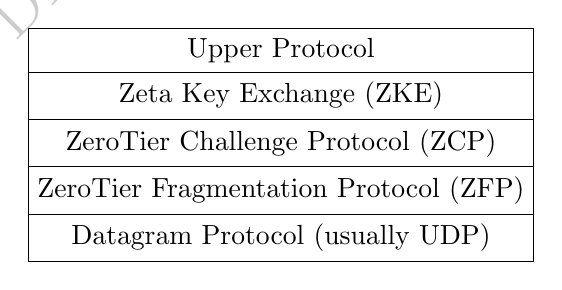
\begin{tikzpicture}[stack/.style={rectangle split, rectangle split parts=#1,draw, anchor=center}]
		\node[stack=5]  {
		\nodepart{one}Upper Protocol
		\nodepart{two}Zeta Key Exchange (ZKE)
		\nodepart{three}ZeroTier Challenge Protocol (ZCP)
		\nodepart{four}ZeroTier Fragmentation Protocol (ZFP)
		\nodepart{five}Datagram Protocol (usually UDP)
		};
	\end{tikzpicture}
\end{figure}

The next section will be dedicated to describing ZKE in explicit detail. We will be making heavy use of common mathematical notions and notation surrounding Deterministic Finite Automata, State Machines and AKE security. The goal with this section is to describe ZKE at a level of detail necessary both to allow someone to implement ZKE, and to aide future mathematical analysis of ZKE.

\begin{definition}[ZKE packet types]
	We define 8 different packet types that are essential for the functioning of ZKE.
	\begin{itemize}
		\item $X_1$: This packet type contains the first message of Noise XK. It is identified internally with packet type number `0'.
		\item $X_2$: This packet type contains the second message of Noise XK. It is identified internally with packet type number `1'.
		\item $X_3$: This packet type contains the third message of Noise XK. It is identified internally with the number packet type number `2'.
		\item $C_1$: This packet type confirms that the remote party has completed the Noise handshake. It is identified internally with packet type number `3'.
		\item $C_2$: This packet type acknowledges that packet type $C_1$ has been received, so the remote peer can stop resending packet $C_1$. It is identified internally with packet type number '4'.
		\item $K_1$: This packet type contains the first message of Noise KK. It is identified internally with packet type number `5'.
		\item $K_2$: This packet type contains the second message of Noise KK. It is identified internally with packet type number `6'.
	\end{itemize}
	In addition, there are 3 packet types which the upper protocol can cause to be sent, but are non-essential to the protocol. These will not be sent unless the upper protocol explicitly calls for them to be sent.
	\begin{itemize}
		\item $D$: This packet type confirms that Bob has completed the Noise handshake, but is refusing to connect to Alice. It is identified internally with packet type number `7'.
		\item $P$: This packet type contains a payload of data for the upper protocol to send and receive. It is identified internally with packet type number `8'.
	\end{itemize}
\end{definition}

\begin{figure}[!ht]
	\caption{Handshake Hello $X_1$ -- This is the packet structure of the first packet Alice sends to Bob. It conforms to the message structure required by the Noise protocol.}\label{packet:handshake_hello}
	\centering
	\begin{bytefield}[bitwidth=5.5em]{4}
		\begin{rightwordgroup}{Noise XK\\Prologue}
			\wordbox{1}{\texttt{key\_id} (4 bytes)}
		\end{rightwordgroup} \\
		\wordbox{2}{\texttt{e} (49 bytes)} \\
		\wordbox[tlr]{2}{\texttt{e1} (1568 bytes)} \\
		\bitbox[blr]{2}{} & \bitbox{2}{\texttt{e1\_tag} (16 bytes)} \\
		\begin{rightwordgroup}{Noise XK\\Payload}
			\wordbox{2}{$\texttt{rf}_1$ (optional 32 bytes)} \\
			\wordbox{2}{$\texttt{rf}_2$ (optional 32 bytes)} \\
			\wordbox{1}{\texttt{rf\_tag} (16 bytes)}
		\end{rightwordgroup} \\
	\end{bytefield}
\end{figure}

\begin{figure}[!ht]
	\caption{Handshake Response $X_2$ -- Bob sends this packet in response to Alice's Hello packet. It also conforms to the message structure of the Noise protocol. All packets in ZKE do.}\label{packet:handshake_response}
	\centering
	\begin{bytefield}[bitwidth=5.5em]{4}
		\wordbox{2}{\texttt{e} (49 bytes)} \\
		\wordbox[tlr]{2}{\texttt{ekem1} (1568 bytes)} \\
		\bitbox[blr]{2}{} & \bitbox{2}{\texttt{ekem1\_tag} (16 bytes)} \\
		\begin{rightwordgroup}{Noise XK\\Payload}
			\wordbox[tlr]{2}{\texttt{key\_id} (4 bytes)} \\
			\bitbox[blr]{2}{} & \bitbox{2}{\texttt{key\_id\_tag} (16 bytes)}
		\end{rightwordgroup} \\
	\end{bytefield}
\end{figure}

\begin{figure}[!ht]
	\caption{Handshake Completion $X_3$ -- This is the packet structure of the final message of Noise XK, which Alice sends to Bob.}\label{packet:handshake_complete}
	\centering
	\begin{bytefield}[bitwidth=6em]{4}
		\wordbox[tlr]{2}{\texttt{s} (49 bytes)} \\
		\bitbox[blr]{2}{} & \bitbox{2}{\texttt{s\_tag} (16 bytes)} \\
		\begin{rightwordgroup}{Noise XK\\Payload}
			\wordbox[tlr]{2}{\texttt{identity} (variable length)} \\
			\bitbox[blr]{2}{} & \bitbox{2}{\texttt{identity\_tag} (16 bytes)}
		\end{rightwordgroup} \\
	\end{bytefield}
\end{figure}

\begin{figure}[!ht]
	\caption{Key Confirmation $C_1$, Acknowledgement $C_2$, and Session Rejection $D$ -- These three packet types have the same packet structure. They just contain a MAC to confirm both peers have completed the handshake.}\label{packet:key_conf}
	\centering
	\begin{bytefield}[bitwidth=5em]{4}
		\wordbox{1}{\texttt{kek\_tag} (16 bytes)}
	\end{bytefield}
\end{figure}

\begin{figure}[!ht]
	\caption{Rekey Initiation $K_1$, and Rekey Completion $K_2$ -- Both types of Noise KK rekeying packets have the same structure.}\label{packet:rekey}
	\centering
	\begin{bytefield}[bitwidth=5.5em]{4}
		\wordbox{2}{\texttt{e} (49 bytes)} \\
		\begin{rightwordgroup}{Noise KK\\Payload}
			\wordbox[tlr]{2}{\texttt{key\_id} (4 bytes)} \\
			\bitbox[blr]{2}{} & \bitbox{2}{\texttt{key\_id\_tag} (16 bytes)}
		\end{rightwordgroup} \\
		\wordbox{1}{\texttt{kek\_tag} (16 bytes)}
	\end{bytefield}
\end{figure}

\begin{figure}[!ht]
	\caption{Data Transport Packet $P$ -- This is the structure of packets containing payloads of data from the upper protocol.}\label{packet:transport}
	\centering
	\begin{bytefield}[bitwidth=5.5em]{4}
		\begin{rightwordgroup}{Noise\\Transport\\Payload}
			\wordbox[tlr]{2}{\texttt{payload} (variable length)} \\
			\bitbox[blr]{2}{} & \bitbox{2}{\texttt{tag} (16 bytes)}
		\end{rightwordgroup} \\
	\end{bytefield}
\end{figure}

\begin{figure}[!ht]
	\caption{The Zeta Key Exchange in ideal conditions.}
	\centering
	\begin{sequencediagram}
		\newinst{a}{Alice}
		\newinst[5]{b}{Bob}
		\mess{a}{Handshake Hello, $X_1$}{b}
		\mess{b}{Handshake Response, $X_2$}{a}
		\mess{a}{Handshake Completion, $X_3$}{b}
		\mess{b}{Key Confirmation, $C_1$}{a}
		\mess{a}{Acknowledgement, $C_2$}{b}
		\mess{a}{Data transport, $P$}{b}
		\mess{b}{Data transport, $P$}{a}
		\begin{sdblock}{Rekeying}{Repeat every hour}
			\mess{a}{Rekey Initiation, $K_1$}{b}
			\mess{b}{Rekey Completion, $K_2$}{a}
			\mess{a}{Key Confirmation, $C_1$}{b}
			\mess{b}{Acknowledgement, $C_2$}{a}
		\end{sdblock}
	\end{sequencediagram}
\end{figure}


\subsection{Zeta State Machine}

We model ZKE as two state machines in communication with each other. Each machine will send or resend packets to the remote party based on which state it is in, will only transition state in response to receiving a particular type of packet from the remote party, and will only modify important cryptographic variables during an atomic transition from one state to the next.

At the end of this section we will have defined $\zeta$, which is the high-level state machine that represents both Alice and Bob's side of ZKE.

\begin{definition}[ZKE Automata]\label{def:automata}
	We will first start by defining Deterministic Finite Automata (DFA) $\beta$, which will be the foundation upon which we construct the ZKE state machine. $\beta$ is depicted in \figureref{fig:automata}.

	Let $Q = \{\bot, A_1, B_2, A_3, S_1, S_2, R_1, R_2\}$ be the set of possible states within $\beta$.

	Let $\Sigma = \{X_1, X_2, X_3, K_1, K_2, C_1, C_2, D, \tau, \chi\}$ be the alphabet of packet types $\beta$ can send and receive, as well as special symbols $\tau$ and $\chi$.

	$\tau$ is not a packet type, but rather a representation of a transition being triggered by a state ``timing out''. All states besides $\bot$ in ZKE have a timeout timer that begins when the state is entered, and if the machine does not transition state, the timer will go off and trigger some state transition.

	$\chi$ represents the event that the actual computer process running ZKE is restarted. For completeness' sake we need to account for all possible times at which ZKE could restart and lose all volatile memory. We have designed ZKE to have the property that it can always gracefully recover from a sudden restart.

	Let $\delta: Q\times\Sigma\to Q$ be the transition function. $\delta$ has the following special transitions:
	\begin{multicols}{3}
		\begin{itemize}
			\item $\delta(\bot, \tau)=A_1$.
			\item $\delta(\bot, X_1)=B_2$.
			\item $\delta(A_1, X_2)=A_3$.
			\item $\delta(A_1, \tau)=A_1$.
			\item $\delta(B_2, X_3)=S_1$.
			\item $\delta(B_2, \tau)=\bot$.
			\item $\delta(A_3, C_1)=S_2$.
			\item $\delta(A_3, D)=\bot$.
			\item $\delta(A_3, \tau)=A_1$.
			\item $\delta(S_1, C_2)=S_2$.
			\item $\delta(S_1, \tau)=\bot$.
			\item $\delta(S_2, \tau)=R_1$.
			\item $\delta(S_2, K_1)=R_2$.
			\item $\delta(R_1, K_1)=R_2$.
			\item $\delta(R_1, K_2)=S_1$.
			\item $\delta(R_1, \tau)=\bot$.
			\item $\delta(R_2, C_1)=R_2$.
			\item $\delta(R_2, \tau)=\bot$.
		\end{itemize}
	\end{multicols}
	In addition, for all states $q\in Q,\ \delta(q, \chi) = \bot$, which in other words means that the process restart symbol, $\chi$, transitions all states to the initial state, $\bot$.
	For all transitions of $\delta$ that are not yet specified, they are the identity transition, as in a transition that maps a state to itself.

	$\beta$ contains the transition $\delta(\bot, \tau)=A_1$, but it is important to note $\bot$, being the initial state, does not have any attached timer within ZKE, and will not be triggered automatically. This transition simply represents the upper protocol initiating a session through ZKE. Most upper protocols will attempt to restart sessions on a timer, which is why we chose to represent this unique transition with the $\tau$ symbol.

	Let $\beta=(Q, \Sigma, \delta, \bot, \{S_2\})$ be the ZKE Automata.
\end{definition}

\begin{figure}
	\caption{The ZKE Automata, $\beta$ -- Both sides of a ZSSP session contain a copy of this machine. $A_1$, $B_2$ and $A_3$ are Noise XK states, $S_1$ and $S_2$ are session established states, and $R_1$ and $R_2$ are Noise KK states. Each symbol represents a received packet type, except for $\tau$ which represents a timeout transition. Omitted are the identity and $\chi$ transitions.}\label{fig:automata}
	\centering
	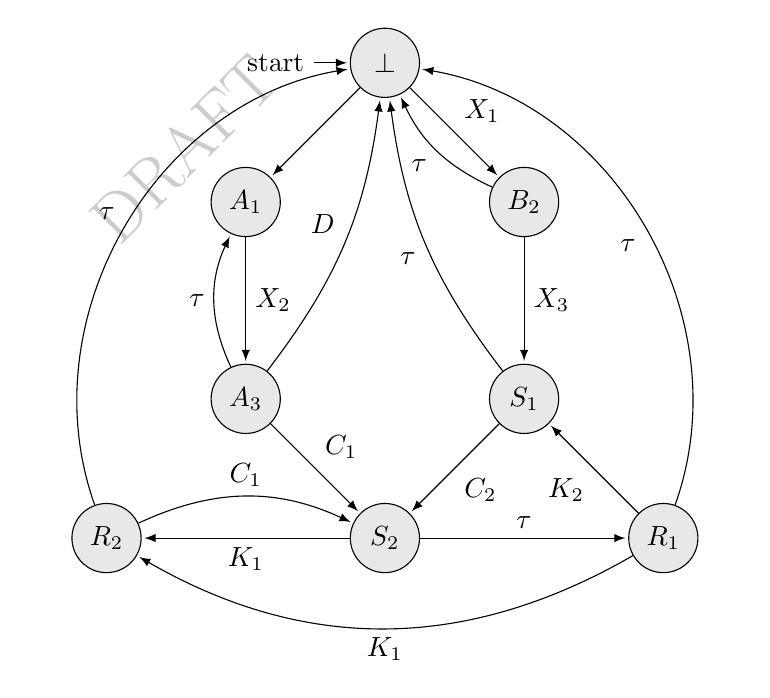
\begin{tikzpicture}[shorten >=1pt,node distance=2.5cm,auto,>=latex]
		\tikzstyle{every state}=[fill={rgb:black,1;white,10}]

		\node[state,initial] (B0) {$\bot$};
		\node[state]         (A1) [below left of=B0] {$A_1$};
		\node[state]         (A2) [below of=A1] {$A_3$};
		\node[state]         (B1) [below right of=B0] {$B_2$};
		\node[state]         (S1) [below of=B1] {$S_1$};
		\node[state]         (S2) [below left of=S1] {$S_2$};
		\node[state]         (R2) [below left of=A2] {$R_2$};
		\node[state]         (R1) [below right of=S1] {$R_1$};

		\path[->]
		(B0) edge                 node {} (A1)
		     edge                 node {$X_1$} (B1)
		(A1) edge                 node {$X_2$} (A2)
		(A2) edge [bend left=25]  node {$\tau$} (A1)
		     edge                 node {$C_1$} (S2)
		     edge [bend right=15] node {$D$} (B0)
		(B1) edge [bend left=20]  node {$\tau$} (B0)
		     edge                 node {$X_3$} (S1)
		(S1) edge [bend left=15]  node {$\tau$} (B0)
		     edge                 node {$C_2$} (S2)
		(S2) edge                 node {$\tau$} (R1)
		     edge                 node {$K_1$} (R2)
		(R1) edge [bend left]     node {$K_1$} (R2)
		     edge                 node {$K_2$} (S1)
		     edge [bend right=50] node {$\tau$} (B0)
		(R2) edge [bend left=25]  node {$C_1$} (S2)
		     edge [bend left=50]  node {$\tau$} (B0);
	\end{tikzpicture}
\end{figure}


\begin{definition}[The Zeta State Machine, $\zeta$]\label{def:state_machine}
	We are going to extend $\beta$ with behaviors and rules that cannot be modelled adequately by DFAs. This new, extended machine will be referred to as $\zeta$, the Zeta state machine. $\zeta$ will retain the core states, alphabet, transition function and initial state as $\beta$, but we are going to add the ability for $\zeta$ to establish a session, send a remote peer encrypted packets, and to process incoming packets.

	$\bot$ is treated as a unique, nondeterministic state within $\zeta$. Internally, $\zeta$ is always in the $\bot$ state. Whenever an input is received that would cause a transition out of the $\bot$ state, $\zeta$ will stay in the $\bot$ state, but spawn a copy of itself that is initialized to the correct transition state, either $A_1$ or $B_2$. If this new instance of $\zeta$ enters the $\bot$ state, it will be deleted from memory. The original  $\zeta$ will still exist in the $\bot$ state, ready to spawn more copies. This is directly analogous to a nondeterministic transition within an NFA. This is how ZKE handles multiple session to a single peer, each session can be considered its own independent instance of the $\zeta$ state machine, running concurrently with each other. If we are only interested in considering one session to one peer, we can safely ignore this rule.

	When $\zeta$ is in a particular state, it chooses specific packet types from the alphabet to send to the remote peer. The remote peer will also be represented by a separately running instance of $\zeta$. When a peer successfully receives a packet, it feeds as input to $\zeta$ and possibly trigger a transition of state. Below is the list of what packet $\zeta$ sends based on which state it is in.
	\begin{itemize}
		\item When entering state $A_1$, packet $X_1$ is created and sent.
		\item When entering state $B_2$, packet $B_2$ is created and sent.
		\item When entering state $A_3$, packet $X_3$ is created and sent.
		\item When entering state $S_1$, packet $D$ or $C_1$ is created and sent.
		\item In state $S_2$, no packet is sent.
		\item When entering state $R_1$, packet $K_1$ is created and sent.
		\item When entering state $R_2$, packet $K_2$ is created and sent.
	\end{itemize}
	\sectionref{sec:trans_alg} discusses how these packets are structured, and what algorithms are used to create and process each packet.

	$\zeta$ has a timer system to automatically and locally trigger state transitions or packet resends. This system exists primarily as a solution to the ``two generals problem''. Since ZKE assumes an out-of-order, lossy transport environment it is necessary to have a system of resending lost messages and timing out those resends, similar to TCP. The ZKE timer system is designed to be lightweight, security focused, and simple. It provides strong guarantees about the maximum amount of time that may pass until certain security critical events, such as completing a handshake or ratcheting a session key, must occur.

	We assume that the underlying computer running $\zeta$ exposes some mechanism for creating a \emph{timer} which can be \emph{set} to some amount of time, and the computer will \emph{trigger} the timer after approximately that amount of real time has passed.
	\begin{itemize}
		\item $\zeta$ runs a single timeout timer that starts whenever any state other than $\bot$ is entered. If any state transition occurs this timer is reset to a new amount of time. If this timer is triggered before a state transition occurs, $\zeta$ gives $\tau$ as input to $\beta$. The timeout timer must never be reset or modified outside of a state transition.
		\item States $A_1$, $B_2$ and $A_3$ always set their timeout timer to 10 seconds.
		\item States $S_1$, $R_1$ and $R_2$ always set their timeout timer to 1 minute.
		\item State $S_2$ sets its timeout timer to a uniform random number in the range 50 minutes to 1 hour. This amount of time is randomly generated each time $\zeta$ enters state $S_2$.
		\item In states $A_1$, $A_3$, $S_1$, $R_1$ and $R_2$, $\zeta$ runs an additional ``resend timer''. Whenever this timer triggers, a copy of the respective packet that this state generated is sent, and the resend timer is reset. Packets $C_1$, $K_1$ and $K_2$ are re-encrypted under the key exchange key \texttt{kek}, and a fresh encryption counter. States $B_2$ and $S_2$ do not have a resend timer and do not resend packets. The resend timer is always set to 1 second.
		\item Any state may trigger timeout early for any reason. In particular it is recommended to timeout state $B_2$ early if memory is being filled with unfinished handshakes. This prevents memory exhaustion attacks.
	\end{itemize}
	The timer system has the property that all timers are generated locally, checked locally, and are never sent ``over the wire''. This has the advantage of making it difficult to impossible for a remote attacker to manipulate a peer's timers. The system has also been intentionally designed to make it impossible for $\zeta$ to ever get indefinitely stuck in one state. If it could, it would open up the possibility that an attacker could intentionally cause this to happen, which would be a form of a DOS attack. The rekeying timer for state $S_1$ is randomized to  deter traffic analysis of ZSSP, and to prevent peers from simultaneously entering state $R_1$, which would be redundant and inefficient.

	It is important to note from this definition that there is no such thing as a ``heartbeat'' in ZKE, nor ZSSP as a whole. ZKE, on its own, does not require ``keep-alive'' messages to be periodically sent between peers. Instead, the only packets ZKE will automatically send are those which are strictly necessary to maintain strong forward secrecy. This makes ZKE ideal for applications where silence is considered a virtue. It is up to the upper protocol to implement a heartbeat or keep-alive system if it is deemed necessary.

	$\zeta$, being a cryptographic protocol, also has many rules relating to how it must cryptographically process incoming or outgoing packets, and how those packets can influence state transitions of $\beta$. Below is a numbered list of all of these rules.
	\begin{enumerate}
		\item Several transitions within $\beta$ have a corresponding algorithm $\zeta$ computes. These are described in \sectionref{sec:trans_alg}. When a transition begins, $\zeta$ computes the corresponding algorithm, and it only allows $\beta$ to transition state if all authentication steps within this algorithm succeed.
		\item If authentication fails specifically during the execution of the Noise XK or Noise KK handshake, this must immediately trigger timeout, $\tau$. Any other form of authentication failure will cause the corresponding packet to be ignored, as if it had never been received.
		\item When transition $\delta(A_1, \tau)=A_1$ or $\delta(A_3, \tau)=A_1$ occurs, $\zeta$ generates a new $X_1$ packet, and does not reuse the previous $X_1$ packet.
		\item The transition, $\delta(R_1, K_1)=R_2$, is only allowed to occur if $\zeta$ acted as Bob, the responder, in the initial Noise XK handshake (i.e. if $\zeta$ has previously been in the $B_2$ state).
		\item If $\zeta$ receives a valid $C_1$ packet while in state $S_1$, $S_2$, $R_1$ or $R_2$, $\zeta$ will reply with a new $C_2$ packet encrypted under the most recently created key exchange key, \texttt{kek}.
		\item $\zeta$ may only send data transport packets on behalf of the upper protocol when in states $S_1$, $S_2$, $R_1$ and $R_2$. Note that this implies a peer may receive data transport packets in states $A_3$, $S_1$, $S_2$, $R_1$ and $R_2$.
		\item If $2^{30}$ or more data transport packets are sent using the same transport key, and $\zeta$ is in state $S_2$, then timeout is triggered early. If $2^{32} - 1$ data transport packets are sent using the same transport key then $\beta$ receives as input symbol $\chi$, which is to say it immediately transitions to state $\bot$ and ends the session.
	\end{enumerate}
\end{definition}

It is not immediately clear why some of the rules in the above list exist, nor what function they might serve in the protocol. For that reason, below is a list of explanations for each processing rule. They are numbered by which rule they are explaining, respectively. Some of these explanation are discussed in further detail in other sections.
\begin{enumerate}
	\item This rule should be fairly self explanatory, in order to provide security ZKE must do authenticated encryption, particularly the authenticated encryption required by the Noise protocol.
	\item This is to conform to the Noise protocol's requirement that the handshake be aborted in the event either peer fails authentication during the handshake. Other than that we want to obey the security principle that inauthentic packets should not trigger any change in state.
	\item  This rule serves a few functions. First and foremost it guarantees that when a handshake is unsuccessful for whatever reason, both Alice and Bob will generate new ephemeral keys. This prevents identical key material from being derived, reducing the risk of catastrophic key reuse. Due to the timer system, this also imposes a strict time limit upon any MitM attack that relies upon intercepting Alice's initial packet. Secondarily, regenerating the $X_1$ packet also regenerates a special nonce value that is used by the ZeroTier Fragmentation Protocol to provide DOS protection.
	\item This is to ensure only one peer can enter state $R_2$ at a time, guaranteeing the other peer stays in state $R_1$. Essentially this rule makes it impossible for both peers to act as Bob at the same time in a Noise KK handshake, which would lock-up a session if it were allowed to happen.
	\item The remote peer will continue to resend $C_1$ packets until it receives a $C_2$ packet. Since $C_2$ packets are not resent, they have to be sent as an acknowledgement packet to every received $C_1$ packet. Otherwise the remote peer might never transition to state $S_2$.
	\item Data transport clearly cannot occur in states $\bot$, $A_1$ and $B_2$, because no Noise key has been established. Alice does obtain a Noise key when they enter state $A_3$. However, for reliability, we want to give Bob an opportunity to refuse connection with Alice based on their static key and identity, and we want to make sure out of order data will be decryptable by Bob. For the sake of improved forward secrecy, we also want to make sure both parties have confirmed a new ratchet fingerprint and ratchet key before they begin communicating. Otherwise, by preventing Bob from ever receiving packet $X_3$, an attacker can cause Alice and Bob to always use the same ratchet key.
	\item This is to conform with NIST's requirement that an AES-GCM key never be used more than $2^{32}$ times. It also avoids AES-GCM's weakening security when a large volume of data is encrypted.
\end{enumerate}

\subsection{Background}

The following are the 4 cryptographic primitives ZKE is based upon. We will be abbreviating these algorithms with generic notation in the sections that follow, notation that is defined here.

\newcommand{\HASH}{\algn{HASH}}
\newcommand{\KDF}{\algn{KDF}}
\newcommand{\AEAD}{\algn{AEAD}}
\newcommand{\DHGEN}{\algn{DH-Gen}}
\newcommand{\KEMGEN}{\algn{KEM-Gen}}
\newcommand{\KEMENC}{\algn{KEM-Enc}}
\newcommand{\KEMDEC}{\algn{KEM-Dec}}
\newcommand{\COUNTER}{\algn{Count}}
\newcommand{\KID}{\algn{KID-Gen}}

\begin{definition}[SHA-512 \cite{fips_sha2}]
	Let $\HASH(M)$ be the SHA-512 hashing algorithm, where $M$ is the string input to be hashed. It has a 512-bit output.
\end{definition}

\begin{definition}[KBKDF \cite{fips_kbkdf}]
	Let $\KDF(\textit{K}_{\textit{IN}}, \textit{Label}, \textit{Context}, N)$ be the KBKDF key derivation algorithm, instantiated in HMAC-Counter mode using SHA-512. Variable $\textit{K}_{\textit{IN}}$ is the input key material, $\textit{Label}$ is some static label, $\textit{Context}$ is additional input key material, and $N$ is the number of 512-bit outputs to be produced. $\KDF(\textit{K}_{\textit{IN}}, \textit{Label}, \textit{Context}, N)$ produces as output $(x_1,\ldots,x_N)$, a tuple of $N$ 512-bit outputs.

	Given $i\in \{1,\ldots,N\}$, we will use the notation $\KDF(\textit{K}_{\textit{IN}}, \textit{Label}, \textit{Context}, N)_i$ to refer to the $i$th output of $\KDF$. When assigning a single 512-bit output to a variable or field that is 256-bits in size, it is assumed that the output is being truncated to just the first 256-bits.

	So $k\gets \KDF(x, l, y, 3)_2$ represents computing KBKDF on inputs $\textit{K}_{\textit{IN}}= x,\, \textit{Label}=l,\, \textit{Context}=y$ and $L=3\cdot 512$, and setting variable $k$ equal to bits $512$ to $1023$ of the output. If $k$ is a variable of size 256-bits, then $k$ is set equal to bits $512$ to $767$ of the output.
\end{definition}

\begin{definition}[AES-GCM \cite{fips_aesgcm}]
	Let $\AEAD(K, N, H, M)$ be the AES-GCM Authenticated Encryption with Additional Data algorithm, where $K$ is the encryption key, $N$ is the nonce or IV, $H$ is the additional authentication data, and $M$ is the plaintext message to be encrypted. $\AEAD(K, N, H, M)$ produces as output $c||t$, a ciphertext, $c$, concatenated with its 128-bit (16 byte) authentication tag, $t$.
\end{definition}

\begin{definition}[P384 \cite{fips_p384}]
	Let $\DHGEN()$ be the P384 elliptic curve Diffie-Helman key generation algorithm. $\DHGEN()$ outputs a random keypair, $(x, g^x)$, where $x$ is the private key and $g^x$ is the public key. $g$ is the generator of the P384 elliptic curve group.
\end{definition}

Given $(x, g^x)$ and $(y, g^y)$, two output keypairs from $\DHGEN()$, a \emph{key agreement} between these keys can be performed by computing $(g^x)^y$ or $(g^y)^x$. It is the case that $(g^x)^y=(g^y)^x=g^{xy}$. This value, $g^{xy}$, is considered the output key material of Diffie-Helman key agreement.

\begin{definition}[Kyber1024 \cite{kyber}]
	Let $(\KEMGEN, \KEMENC, \KEMDEC)$ be the Kyber1024 key encapsulation mechanism. $\KEMGEN()$ randomly generates a keypair, $(e_{priv}, e_{pub})$, where $e_{priv}$ is the private key and $e_{pub}$ is the public key. $\KEMENC(e_{pub})$ takes as input a Kyber1024 public key, and outputs the pair $(e_{key}, e_{kem})$, where $e_{key}$ is the symmetric key and $e_{kem}$ is the encapsulated ciphertext of $e_{key}$. $\KEMDEC(e_{priv}, e_{kem})$ takes as input a private key and an encapsulated ciphertext, and outputs $e_{key}$, the decryption of $e_{kem}$. Both \KEMENC and \KEMDEC can output $\bot$, the null value, which implies authentication failure due to invalid input keys.
\end{definition}

\subsection{Transition Algorithms}\label{sec:trans_alg}

With the necessary background established, we can now define the final component of the Zeta state machine, the state transition algorithms. As is described in \definitionref{def:state_machine}, each state transition within $\zeta$ has a corresponding algorithm that must be computed. All of these algorithms are described in this section. They have access to a collection of global variables, defined below.

\begin{itemize}
	\item Persistent ratchet keys $\texttt{rk}_1, \texttt{rk}_2$, to be used as a handshake PSK
	\item Persistent ratchet fingerprints $\texttt{rf}_1, \texttt{rf}_2$, to identify a particular ratchet key
	\item Long term static keypairs $(u, g^u)$ and $(v, g^v)$
	\item Short term randomized key identifiers $\texttt{kid}^\texttt{i}_1, \texttt{kid}^\texttt{i}_2$, to be used for multiplexing between multiple peers
	\item Short term key exchange keys $\texttt{kek}^\texttt{i}_1, \texttt{kek}^\texttt{i}_2$, for authenticating key confirmations and rekeying
	\item Short term Noise transport keys $\texttt{nk}^\texttt{i}_1, \texttt{nk}^\texttt{i}_2$, for AEAD encryption of data transport packets
	\item Short term header keys $\texttt{hk}_1, \texttt{hk}_2$, to be used by the ZeroTier fragmentation protocol
	\item Ephemeral keypairs $(x, g^x)$ and $(y, g^y)$
	\item Ephemeral key encapsulation variables $e_{priv}, e_{pub}, e_{key}$ and $e_{kem}$
	\item Ephemeral Noise chaining keys, $c$ and $c'$
	\item Ephemeral Noise encryption keys, $k$ and $k'$
	\item Ephemeral Noise handshake hashes, $h$ and $h'$
	\item Temporary ratchet key and fingerprint $\texttt{rk}'\andb \texttt{rf}'$, used so Bob can complete Noise XK before knowing Alice's identity.
	\item Role identifier $\texttt{r}$, used so peers are aware whether they were Alice or Bob in Noise XK
	\item Confirmed key index $\texttt{i}$, used so peers know the most recently confirmed Noise key.
\end{itemize}

All of these variables are independent \emph{per instance of} $\zeta$. So each instance of $\zeta$ stores a unique and independent set of these variables, and they are never shared between separate instances of $\zeta$. The persistent state variables $\texttt{rk}$ and $\texttt{rf}$ are a partial exception to this rule, as they can be accessed by multiple instances of $\zeta$ over time. However each of these instances must be associated with a single, unique remote peer, and two instances of $\zeta$ must never access the same set of persistent state variables at the same time.

What constitutes a ``single, unique remote peer'' is up to the upper protocol to decide. Usually remote peers are identified and differentiated by their static public keys ($g^u$ or $g^v$). However ZKE does not strictly enforce a one-to-one relationship between static public keys and identity specifically so the upper protocol is able to rotate the static public keys of peers.

\begin{definition}[Session Counter]
	Every instance of $\zeta$ contains a single monotonically increasing counter, that is initialized to 0. We will use the notation $\COUNTER()$ to represent incrementing this counter by 1 and returning the previous counter value.

	So the very first call to $\COUNTER()$ within $\zeta$ will return 0, the second call will return 1, and so on.

	It is assumed that that output of $\COUNTER()$, the counter value, will be used as an AES-GCM nonce. When a remote peer decrypts an AES-GCM ciphertext that uses a counter value nonce, they must first statefully check that this counter has never been received before, and fail authentication if it has been replayed.
\end{definition}

ZKE uses a 64-bit (8 byte) counter, but AES-GCM uses a 96-bit (12 byte) nonce/IV. The Noise protocol does specify that, in order to use a counter value as an AES nonce, it should be encoded as a big-endian integer with 4 bytes of zero padding to the left of it. However, for good reason, we have decided to utilize the rightmost byte of that 4 byte padding to store the packet type number, as depicted in \figureref{fig:nonce}. This accomplishes two goals. First it explicitly authenticates the packet type of a packet, which makes it infeasible for an attacker to change the packet type field of a header without triggering an authentication failure. We could have used the additional authentication data parameter of AES-GCM to accomplish this, but the Noise protocol already makes extensive use of this parameter. Second, this nonce construction reduces the risk of catastrophic nonce reuse due to implementation error, specifically during key exchanges. While a correctly implemented counter would be sufficient for security, this adds an extra layer of defence. Given a packet type number $p$, and a counter value $c$, we will use the notation $p||c$ to represent this nonce construction.

\begin{figure}
	\caption{Construction of the AES-GCM 96-bit nonce/IV.}\label{fig:nonce}
	\centering
	\begin{bytefield}[bitwidth=3.5em]{10}
		\bitbox{3}{\texttt{0x000000} (3 bytes)} &
		\bitbox{2}{\texttt{type} (1 byte)} &
		\bitbox{6}{\texttt{counter} (big-endian 64-bit integer)}
	\end{bytefield}
\end{figure}

\begin{definition}[Key Id Generation]
	\algn{KID-Gen} is a stateful algorithm that outputs a locally unique, uniform random 32-bit string. The output of this algorithm will be used as the \emph{key id} for a session key, allowing the local peer to multiplex many keys for many remote peers simultaneously. The output of $\algn{KID-Gen}()$ must be locally unique from all other key ids currently in use. $\algn{KID-Gen}()$ may only repeat an output if that output is currently not being used as a key id.
\end{definition}


\begin{definition}[Persistent State]
	The variables $\texttt{rk}$ and $\texttt{rf}$ are considered the \emph{persistent state} of ZKE. The values stored in these variables are not lost when a session ends, and can be \emph{restored} at any time to initiate a new session.

	$\texttt{rk}$ is a tuple of up to two 256-bit \emph{ratchet keys}. Similarly, $\texttt{rf}$ is a tuple of up to two 256-bit \emph{ratchet fingerprints}. $\texttt{rk}$ is initialized to $(0^{256}, \bot)$ and $\texttt{rf}$ is initialized to $(\varepsilon, \bot)$.

	If two peers are in persistent mode, and wish to connect for the first time, they may use a preshared one time password, $p$, to do so. $p$ should be a randomized string, and it must not be correlated with the identity of either peer. If a one time password is being used then $r\gets \KDF(p, \texttt{"ZSSP\_OTP\_TO\_RATCHET"}, \varepsilon, 2)$ must be computed. Both peers then initialize $\texttt{rk}$ to $(r_1, \bot)$ and $\texttt{rf}$ to $(r_2, \bot)$.
\end{definition}

$\bot$ represents the ``null'' value. When a variable is set to $\bot$, it means whatever was previous stored within the variable is being permanently deleted from memory. All variables are initialized to $\bot$ unless otherwise stated. $\varepsilon$ is the empty string.

It is assumed that prior to any usage of ZKE, Alice and Bob will generate their static keypairs with $\DHGEN()$. It is also assumed that Alice already knows Bob's public key, $g^v$, prior to any attempt to connect to Bob. Bob does not necessarily know Alice's public key.

\begin{table}
	\caption{Intermediate Values of the Noise XKhfs+psk2 and the Noise KKpsk0 Handshakes \cite{noise_protocol} \cite{noise_hfs} -- $(u, g^u)$ and $(v, g^v)$ are respectively the static keypairs of Alice and Bob within \emph{the current Noise handshake}, and the label $L=\texttt{"ZSSP"}$. The ciphertext of packets is hashed and not the plaintext. The following transition algorithms implicitly compute and have access to the values described here. This syntax for defining cryptographic variables comes from Benjamin Dowling et.~al.~\cite{wireguard_analysis}}
	\centering
	\renewcommand{\arraystretch}{1.05}
	\begin{tabular}{ | c | c | c | c | }
		\hline
		$i$ & Chaining Key, $c_i$ & Encryption Key, $k_i$ & Handshake Hash, $h_i$ \\
		\hline
		0 & $\texttt{protocol\_name}$ & - & $\texttt{protocol\_name}$ \\
		1 & - & - & $\HASH(h_0||\texttt{kid}_1)$ \\
		2 & - & - & $\HASH(h_1||g^v)$ \\
		3 & $\KDF(g^x, L, c_0, 2)_1$ & - & $\HASH(h_2||g^x)$ \\
		4 & $\KDF(g^{xv}, L, c_3, 2)_1$ & $\KDF(g^{xv}, L, c_3, 2)_2$ & - \\
		5 & - & - & $\HASH(h_3||X_1\texttt{.e1})$ \\
		6 & - & - & $\HASH(h_4||X_1\texttt{.rf})$ \\
		\hline
		7 & $\KDF(g^y, L, c_4, 2)_1$ & - & $\HASH(h_6||g^y)$ \\
		8 & $\KDF(g^{xy}, L, c_7, 2)_1$ & $\KDF(g^{xy}, L, c_7, 2)_2$ & - \\
		9 & $\KDF(e_{key}, L, c_8, 2)_1$ & - & $\HASH(h_7||X_2\texttt{.ekem1})$ \\
		10 & $\KDF(\texttt{rk}', L, c_9, 3)_1$ & $\KDF(\texttt{rk}', L, c_9, 3)_3$ & $\HASH(h_9||\KDF(\texttt{rk}', L, c_9, 3)_2)$ \\
		11 & - & - & $\HASH(h_{10}||X_2\texttt{.key\_id})$ \\
		\hline
		12 & - & - & $\HASH(h_{11}||X_3\texttt{.s})$ \\
		13 & $\KDF(g^{uy}, L, c_{10}, 2)_1$ & $\KDF(g^{uy}, L, c_{10}, 2)_2$ & - \\
		14 & - & - & $\HASH(h_{12}||X_3\texttt{.identity})$ \\
		\hline
		\hline
		$i$ & Chaining Key, $c_i'$ & Encryption Key, $k_i'$ & Handshake Hash, $h_i'$ \\
		\hline
		0 & $\texttt{protocol\_name}'$ & - & $\texttt{protocol\_name}'$ \\
		1 & - & - & $\HASH(h_0'||g^u)$ \\
		2 & - & - & $\HASH(h_1'||g^v)$ \\
		3 & $\KDF(\texttt{rk}_1, L, c_0', 3)_1$ & - & $\HASH(h_2'||\KDF(\texttt{rk}_1, L, c_0', 3)_2)$ \\
		4 & $\KDF(g^x, L, c_3', 2)_1$ & - & $\HASH(h_3'||g^x)$ \\
		5 & $\KDF(g^{xv}, L, c_4', 2)_1$ & - & - \\
		6 & $\KDF(g^{uv}, L, c_5', 2)_1$ & $\KDF(g^{uv}, L, c_5', 2)_2$ & - \\
		7 & - & - & $\HASH(h_4'||K_1\texttt{.key\_id})$ \\
		\hline
		8 & $\KDF(g^y, L, c_6', 2)_1$ & - & $\HASH(h_7'||g^y)$ \\
		9 & $\KDF(g^{xy}, L, c_8', 2)_1$ & - & - \\
		10 & $\KDF(g^{uy}, L, c_9', 2)_1$ & $\KDF(g^{uy}, L, c_9', 2)_2$ & - \\
		11 & - & - & $\HASH(h_8'||K_2\texttt{.key\_id})$ \\
		\hline
	\end{tabular}
\end{table}

We will not be going into detail how each packet is decrypted. All decryption within ZKE is either a straightforward implementation of Noise XK and Noise KK decryption, or otherwise a trivial application of AEAD decryption using AES-GCM. We will be assuming each packet is decrypted in-place, as in we will be reusing the local variable that referred to the encrypted packet to also refer to the decrypted packet.

If packet decryption fails because the AEAD MAC is inauthentic, this is considered authentication failure. Unless otherwise stated, if authentication fails all of the following algorithms immediately cease execution and returns an authentication failure error.

Prior to the execution of any of the following algorithms, $\zeta$ will check if it is in the correct state, if it is allowed to perform the related state transition, that the received key id matches the expected key id, and that the packet has the correct type number. If any of these checks fail execution is aborted and the packet is ignored.

\begin{algorithm}\label{alg:x1}
	\caption{Transition $\delta(\bot, \tau)=A_1$ -- Alice creates and sends a ``Hello'' packet to initialize a session with Bob, \figureref{packet:handshake_hello}. Alice knows Bob's static public key, $g^v$, prior to execution. By sending a Hello packet to Bob, Alice is implicitly trusting Bob.}
	\begin{algorithmic}
		\Require $g^v$
		\State $\textbf{Restore } (\texttt{rk}, \texttt{rf}) \text{ based on Bob's identity}$
		\State $(x, g^x) \gets \DHGEN()$
		\State $(e_{priv}, e_{pub}) \gets \KEMGEN()$
		\State $\texttt{kid}^1_1 \gets \KID()$
		\State $X_1\texttt{.key\_id} \gets \texttt{kid}^1_1$
		\State $X_1\texttt{.e} \gets g^x$
		\State $X_1\texttt{.e1} \gets \AEAD(k_4, 0||0, h_3, e_{pub})$
		\State $X_1\texttt{.rf} \gets \AEAD(k_4, 0||1, h_5, \texttt{rf})$
		\State $\texttt{hk} \gets \KDF(h_6, \texttt{"ASKH"}, c_4, 2)$
		\State $c \gets X_1\texttt{.rf\_tag}\ \text{(last 8 bytes)}$
		\State $\textbf{Send } (0,\ 0||c,\ X_1)$
	\end{algorithmic}
\end{algorithm}

The ratchet fingerprint, \texttt{rf}, is a sacrificial ASK that does nothing more than uniquely identify the ratchet key it was derived with. This makes it possible for Bob to immediately identify Alice given just their Hello packet, if their Hello includes a ratchet fingerprint. Bob can configure ZKE to only reply to peers that have recognized ratchet fingerprints, thereby making ZKE entirely silent to everyone who does not have an authentic ratchet fingerprint. An attacker can record an authentic peer's Hello packet and replay it, but Bob will only reply to this replayed packet for a short period of time, until that ratchet fingerprint is replaced. This is superior to Noise XK's normal Hello packet security properties, which have no authentication and are vulnerable to replay.

Including the ratchet fingerprint in the Hello packet does not compromise identity hiding, because the ratchet fingerprint is replaced with every single handshake. In the event that Bob's private keys are compromised, and all ratchet fingerprints used in Hello packets to Bob can be decrypted, all an attacker would see are several indistinguishable 256-bit strings. The one exception is if a peer reuses the same ratchet fingerprint. This would allow an attacker who has compromised Bob's static private key to learn that two Hello packets come from the same peer, but this does not given any information about that peer's static keys or identity. Ratchet fingerprints in normal operation are never reused, this can only happen if the initial Noise XK handshake is aborted before completion, preventing one or more of the participating peers from confirming a new ratchet fingerprint.

\begin{algorithm}
	\caption{Transition $\delta(\bot, X_1)=B_2$ -- Bob has received Alice's Hello packet and replies with the second message of Noise XK, \figureref{packet:handshake_response}. Input $\pi_1$ is a security flag, a bit set by the upper protocol. Bob will only allow Alice to connect with zero persistent state if $\pi_1=0$. If Alice sent an unrecognized ratchet fingerprint and $\pi_1=0$, instead of rejecting Alice's session, Bob will ask Alice if they would like to connect with zero persistent state. ZKE has superior security properties when $\pi_1=1$, but usability suffers.}\label{alg:recv_x1}
	\begin{algorithmic}
		\Require $(0,\ 0||c,\ X_1),\, \pi_1,$
		\If{$c \neq X_1\texttt{.rf\_tag}$ (last 8 bytes)}
			\State \textbf{Fail authentication}
		\EndIf
		\State $\textbf{Decrypt } X_1$ according to Noise XK
		\State $\texttt{rf}' \gets X_1\texttt{.rf}_1$
		\State $\textbf{Restore } \texttt{rk}' \text{ based on } \texttt{rf}'$
		\If{$\texttt{rk}' = \bot$}
			\State $\texttt{rf}' \gets X_1\texttt{.rf}_2$
			\State $\textbf{Restore } \texttt{rk}' \text{ based on } \texttt{rf}'$
			\If{$\texttt{rk}' = \bot$}
				\If{$\pi_1=1$}
					\State \textbf{Fail authentication}
				\Else
					\State $\texttt{rf}' \gets \varepsilon$
					\State $\texttt{rk}' \gets 0^{256}$
				\EndIf
			\EndIf
		\EndIf
		\State $\texttt{hk} \gets \KDF(h_6, \texttt{"ASKH"}, c_4, 2)$
		\State $\texttt{kid}^1_1 \gets X_1\texttt{.key\_id}$
		\State $\texttt{kid}^1_2 \gets \KID()$
		\State $(y, g^y) \gets \DHGEN()$
		\State $(e_{key}, e_{kem}) \gets \KEMENC(e_{pub})$
		\State $X_2\texttt{.e} \gets g^y$
		\State $X_2\texttt{.ekem1} \gets \AEAD(k_8, 1||0, h_7, e_{kem})$
		\State $X_2\texttt{.key\_id} \gets \AEAD(k_{10}, 1||0, h_{10}, \texttt{kid}^1_2)$
		\State $c \gets X_2\texttt{.key\_id\_tag}\ \text{(last 3 bytes)}$
		\State $\textbf{Send } (\texttt{kid}^1_1,\ 1||c,\ X_2)$
	\end{algorithmic}
\end{algorithm}

\begin{algorithm}
	\caption{Transition $\delta(A_1, X_2)=A_3$ -- Alice has received Bob's reply and can now send a Handshake Completion packet, \figureref{packet:handshake_complete}. Input $\pi_2$ is a security flag, a bit set by the upper protocol. Bob may ask Alice if they would like to connect with zero persistent state instead of the current persistent state. If $\pi_2=0$ then Alice will accept this request, and reset their ratchet keys. Input \texttt{identity} is an arbitrary string provided by the upper protocol. It is expected to contain some form of cryptographic identifier or certificate for this peer, but it could also be the empty string.}\label{alg:recv_x2}
	\begin{algorithmic}
		\Require $(\texttt{kid}^1_1,\ 1||c,\ X_2),\, \pi_2,\, \texttt{identity}$
		\If{$c \geq 2^{24} \orb c \neq X_2\texttt{.key\_id\_tag}$ (last 3 bytes)}
			\State \textbf{Fail authentication}
		\EndIf
		\State $\textbf{Decrypt } X_2$ according to Noise XK using PSK $\texttt{rk}_1$
		\State $i \gets 1$
		\If{$X_2$ failed authentication}
			\State $\textbf{Decrypt } X_2$ according to Noise XK using PSK $\texttt{rk}_2$
			\State $i \gets 2$
			\If{$X_2$ failed authentication}
				\If{$\pi_2=1$}
					\State \textbf{Fail authentication}
				\Else
					\State $\textbf{Decrypt } X_2$ according to Noise XK using PSK $0^{256}$
					\State \textbf{Warn} the upper protocol that Bob does not have the ratchet key
				\EndIf
			\EndIf
		\EndIf
		\State $\texttt{kid}^1_2 \gets X_2\texttt{.key\_id}$
		\State $X_3\texttt{.s} \gets \AEAD(k_{10}, 2||1, h_{11}, g^u)$
		\State $X_3\texttt{.identity} \gets \AEAD(k_{13}, 2||0, h_{12}, \texttt{identity})$
		\State $\texttt{kek}^1 \gets \KDF(h_{14}, \texttt{"ASKK"}, c_{13}, 2)$
		\State $\texttt{nk}^1 \gets \KDF(\varepsilon, L, c_{13}, 2)$
		\State $(\texttt{rk}_2, \texttt{rf}_2) \gets (\texttt{rk}_i, \texttt{rf}_i)$
		\State $(\texttt{rk}_1, \texttt{rf}_1) \gets \KDF(h_{14}, \texttt{"ASKR"}, c_{13}, 2)$
		\State $\texttt{r} \gets 1$
		\State $\texttt{i} \gets 0$
		\State $\textbf{Send } (\texttt{kid}^1_2,\ 2||0,\ X_3)$
	\end{algorithmic}
\end{algorithm}

Packet types $X_2$ and $K_1$ represent the second to last message of Noise XK and Noise KK. The remote peer will not have derived the Noise key yet, so if this peer attempted to encrypt with this key immediately, there is a risk its packets will arrive out of order and be undecryptable. Receiving a valid $C_1$ packet from the remote peer confirms that they have successfully derived the correct Noise key, which signals it can now be reliably used for encryption.

Similarly, the new ratchet key and fingerprint will not have been derived by the remote peer yet. So this peer will have to save these keys to persistent storage, but not yet delete the previous ratchet key and fingerprint until the remote peer sends a key confirmation. This means that for a brief period of time Alice has two sets of ratchet keys and fingerprints saved, instead of just one. We want to make sure Alice and Bob never have more than two of these keys saved at a time. So during the Noise XK handshake if Alice has two sets of keys and fingerprints, they must send both fingerprints to Bob, and delete the key and fingerprint that Bob chooses not to use as the PSK.

\begin{algorithm}
	\caption{Transition $\delta(B_2, X_3)=S_1$ -- Bob receives the final packet of Noise XK. Input $\algn{Accept}$ is a function provided by the upper protocol that takes as input Alice's identity and outputs security flags $(\pi_3, \pi_4)$, $\pi_3$ can be $\bot$. If $\pi_3=\bot$, Bob will reject Alice's session. If $\pi_3=1$, and Bob is aware of a ratchet key Alice should have, but Alice is not connecting with it, Bob will reject Alice's session (similar to when $\pi_2=1$). If Bob rejects Alice's session and $\pi_4 = 0$, Bob will send a packet to Alice explicitly rejecting their session.}\label{alg:recv_x3}
	\begin{algorithmic}
		\Require $(\texttt{kid}_2,\ 2||0,\ X_3),\,\algn{Accept}$
		\State $\textbf{Decrypt } X_3$ according to Noise XK
		\State $\texttt{kek}^1 \gets \KDF(h_{14}, \texttt{"ASKK"}, c_{13}, 2)$
		\State $c \gets \COUNTER()$
		\State $(\pi_3, \pi_4) \gets \algn{Accept}(X_3\texttt{.s}, X_3\texttt{.identity})$
		\If{$\pi_3 \neq \bot$}
			\State $\textbf{Restore } (\texttt{rk}, \texttt{rf}) \text{ based on } (X_3\texttt{.s}, X_3\texttt{.identity})$
			\If{$(\texttt{rf}', \texttt{rk}') \neq (\texttt{rf}_1, \texttt{rk}_1) \andb (\texttt{rf}', \texttt{rk}') \neq (\texttt{rf}_2, \texttt{rk}_2)$}
				\If{$\pi_3 = 0 \andb \texttt{rf}' = \varepsilon$}
					\State \textbf{Warn} the upper protocol that Alice does not have the ratchet key
				\Else
					\If{$\pi_4 = 0$}
						\State $D\texttt{.kek\_tag} \gets \AEAD(\texttt{kek}^1_1, 7||c, \varepsilon, \varepsilon)$
						\State $\textbf{Send } (\texttt{kid}_1,\ 7||c,\ D)$
					\EndIf
					\State \textbf{Fail authentication}
				\EndIf
			\EndIf
			\State $\texttt{nk}^1 \gets \KDF(\varepsilon, L, c_{13}, 2)$
			\State $(\texttt{rk}_2, \texttt{rf}_2) \gets \bot$
			\State $(\texttt{rk}_1, \texttt{rf}_1) \gets \KDF(h_{14}, \texttt{"ASKR"}, c_{13}, 2)$
			\State $\texttt{r} \gets 2$
			\State $\texttt{i} \gets 1$
			\State $C_1\texttt{.kek\_tag} \gets \AEAD(\texttt{kek}^1_1, 3||c, \varepsilon, \varepsilon)$
			\State $\textbf{Send } (\texttt{kid}_1,\ 3||c,\ C_1)$
		\Else
			\If{$\pi_4=0$}
				\State $D\texttt{.kek\_tag} \gets \AEAD(\texttt{kek}^1_1, 7||c, \varepsilon, \varepsilon)$
				\State $\textbf{Send } (\texttt{kid}_1,\ 7||c,\ D)$
			\EndIf
			\State \textbf{Fail authentication}
		\EndIf
	\end{algorithmic}
\end{algorithm}

When packet $X_3$ is received, Bob might refuse to start a session with Alice based on their static key and identity. The preferred way for Bob to do this is to simply do nothing, and ignore Alice's packets. This would follow the ``silence is a virtue" principle of security. However there are some applications where, usually for UX reasons, Alice needs to be able tell apart having a bad connection with Bob from Bob rejecting Alice's identity. If Bob always goes silent Alice has no reliable way to tell these two situations apart. Since both Bob and Alice have the key exchange key at this point in the handshake, it was a very natural and secure extension of the protocol to allow Bob to notify Alice that the session has been refused.

Packet types $X_3$ and $K_2$ represent the final messages of Noise XK and Noise KK, respectively. The peer who receives these packets can be sure that the remote peer has derived an identical Noise key already, and so the new key can be reliably used immediately.

\begin{algorithm}
	\caption{Transition $\delta(A_3, C_1)=S_2$ and $\delta(R_2, C_1)=S_2$ -- A key confirmation for either the Noise XK initial handshake or Noise KK rekeying has been received. This peer must send an Acknowledgement, \figureref{packet:key_conf}, to let the remote peer know that it has been received.}\label{alg:key_conf}
	\begin{algorithmic}
		\Require $(\texttt{kid}^{\texttt{i} + 1}_{\texttt{r}},\ 3||c,\ C_1)$
		\State $\textbf{Decrypt } C_1$ using $\texttt{kek}^{\texttt{i} + 1}_{\texttt{r}}$
		\State $(\texttt{rk}_2, \texttt{rf}_2) \gets \bot$
		\State $\texttt{i} \gets \texttt{i} + 1$
		\State $c \gets \COUNTER()$
		\State $C_2\texttt{.kek\_tag} \gets \AEAD(\texttt{kek}^\texttt{i}_{3 - \texttt{r}}, 4||c, \varepsilon, \varepsilon)$
		\State $\textbf{Send } (\texttt{kid}^\texttt{i}_{3 - \texttt{r}},\ 4||c,\ C_2)$
	\end{algorithmic}
\end{algorithm}

Packet types $C_2$ and $D$ have trivial transition algorithms. They merely decrypt the received packet with the most recent key exchange key, $\texttt{kek}^\texttt{i}_\texttt{r}$. If authentication succeeds then $\zeta$ transitions state.

\begin{algorithm}
	\caption{Transition $\delta(S_2, \tau)=R_1$ -- This peer, whom will be henceforth be referred to as Alice, has decided to initiate rekeying. They create and send a Rekey Initiation packet, \figureref{packet:rekey}, to the remote peer, Bob. The entire Noise KK message is encrypted under the key exchange key for additional security.}
	\begin{algorithmic}
		\State $\texttt{kid}^{\texttt{i} + 1}_\texttt{r} \gets \KID()$
		\State $(x, g^x) \gets \DHGEN()$
		\State $K_1\texttt{.e} \gets g^x$
		\State $K_1\texttt{.key\_id} \gets \AEAD(k_{6}', 5||0, h_{4}, \texttt{kid}^{\texttt{i} + 1}_\texttt{r})$
		\State $c \gets \COUNTER()$
		\State $K_1 \gets \AEAD(\texttt{kek}^\texttt{i}_{3 - \texttt{r}}, 5||c, \varepsilon, K_1)$
		\State $\textbf{Send } (\texttt{kid}^\texttt{i}_{3 - \texttt{r}},\ 5||c,\ K_1)$
	\end{algorithmic}
\end{algorithm}


\begin{algorithm}
	\caption{Transition $\delta(S_2, K_1)=R_2$ and $\delta(R_1, K_1)=R_2$ -- Bob has received Alice's request to rekey and sends a Rekey Completion packet, \figureref{packet:rekey}, in reply. Bob has now finished Noise KK and has obtained a new Noise key. A new pair of key ids are generated so Bob can tell apart packets encrypted with the new key from those encrypted with the previous key.}
	\begin{algorithmic}
		\Require $(\texttt{kid}^\texttt{i}_\texttt{r},\ 5||c,\ K_1)$
		\State $\textbf{Decrypt } K_1$ using $\texttt{kek}^\texttt{i}_\texttt{r}$, and Noise KK
		\State $\texttt{kid}^{\texttt{i} + 1}_{3 - \texttt{r}} \gets K_1\texttt{.key\_id}$
		\State $\texttt{kid}^{\texttt{i} + 1}_\texttt{r} \gets \KID()$
		\State $(y, g^y) \gets \DHGEN()$
		\State $K_2\texttt{.e} \gets g^y$
		\State $K_2\texttt{.key\_id} \gets \AEAD(k_{10}', 6||0, h_{8}, \texttt{kid}^{\texttt{i} + 1}_\texttt{r})$
		\State $c \gets \COUNTER()$
		\State $K_2 \gets \AEAD(\texttt{kek}^\texttt{i}_{3 - \texttt{r}}, 6||c, \varepsilon, K_2)$
		\State $\texttt{kek}^{\texttt{i} - 1} \gets \bot$
		\State $(\texttt{kek}^{\texttt{i} + 1}_{3 - \texttt{r}}, \texttt{kek}^{\texttt{i} + 1}_\texttt{r}) \gets \KDF(h_{11}', \texttt{"ASKK"}, c_{10}', 2)$
		\State $\texttt{nk}^{\texttt{i} - 1} \gets \bot$
		\State $(\texttt{nk}^{\texttt{i} + 1}_{3 - \texttt{r}}, \texttt{nk}^{\texttt{i} + 1}_\texttt{r}) \gets \KDF(\varepsilon, L, c_{10}', 2)$
		\State $(\texttt{rk}_2, \texttt{rf}_2) \gets (\texttt{rk}_1, \texttt{rf}_1)$
		\State $(\texttt{rk}_1, \texttt{rf}_1) \gets \KDF(h_{11}', \texttt{"ASKR"}, c_{10}', 2)$
		\State $\textbf{Send } (\texttt{kid}^\texttt{i}_{3 - \texttt{r}},\ 6||c,\ K_2)$
	\end{algorithmic}
\end{algorithm}


\begin{algorithm}
	\caption{Transition $\delta(R_1, K_2)=S_1$ -- Alice has received Bob's reply and so can also finish Noise KK. They send a Key Confirmation, \figureref{packet:key_conf}, to signal the completion of the handshake. The second to last Noise key is deleted for forward secrecy.}
	\begin{algorithmic}
		\Require $(\texttt{kid}^\texttt{i}_\texttt{r},\ 6||c,\ K_2)$
		\State $\textbf{Decrypt } K_2$ using $\texttt{kek}^\texttt{i}_\texttt{r}$, and Noise KK
		\State $\texttt{kid}^{\texttt{i} + 1}_{3 - \texttt{r}} \gets K_2\texttt{.key\_id}$
		\State $\texttt{kek}^{\texttt{i} - 1} \gets \bot$
		\State $(\texttt{kek}^{\texttt{i} + 1}_\texttt{r}, \texttt{kek}^{\texttt{i} + 1}_{3 - \texttt{r}}) \gets \KDF(h_{11}', \texttt{"ASKK"}, c_{10}', 2)$
		\State $\texttt{nk}^{\texttt{i} - 1} \gets \bot$
		\State $(\texttt{nk}^{\texttt{i} + 1}_\texttt{r}, \texttt{nk}^{\texttt{i} + 1}_{3 - \texttt{r}}) \gets \KDF(\varepsilon, L, c_{10}', 2)$
		\State $(\texttt{rk}_1, \texttt{rf}_1) \gets \KDF(h_{11}', \texttt{"ASKR"}, c_{10}', 2)$
		\State $\texttt{i} \gets \texttt{i} + 1$
		\State $c \gets \COUNTER()$
		\State $C_1\texttt{.kek\_tag} \gets \AEAD(\texttt{kek}^\texttt{i}_{3 - \texttt{r}}, 3||c, \varepsilon, \varepsilon)$
		\State $\textbf{Send } (\texttt{kid}^\texttt{i}_{3 - \texttt{r}},\ 3||c,\ C_1)$
	\end{algorithmic}
\end{algorithm}

We want to minimize the number of Noise keys alive in memory for the sake of perfect forward secrecy, in case the content of a peer's memory is stolen by an attacker. However we have to keep at least the last 2 keys around for reliability. Otherwise a packet that was sent before rekeying could arrive out of order, after the rekey is completed, and not be decryptable.

\begin{algorithm}
	\caption{Data transport send -- The upper protocol has decided to send the remote peer an encrypted payload. Input \texttt{payload} is an arbitrary string provided by the upper protocol.}
	\begin{algorithmic}
		\Require $\texttt{payload}$
		\State $c \gets \COUNTER()$
		\State $P\texttt{.payload} \gets \AEAD(\texttt{nk}^\texttt{i}_{3 - \texttt{r}}, 8||c, \varepsilon, \texttt{payload})$
		\State $\textbf{Send } (\texttt{kid}^\texttt{i}_{3 - \texttt{r}},\ 8||c,\ P)$
	\end{algorithmic}
\end{algorithm}

\begin{algorithm}
	\caption{Data transport received -- A data transport packet has been received. It is decrypted and its payload is given to the upper protocol to handle.}
	\begin{algorithmic}
		\Require $(\texttt{kid}^i_r,\ 8||c,\ P)$
		\State $\textbf{Decrypt } P$ using $\texttt{nk}^i_r$ (if $\texttt{nk}^i_r=\bot$ then authentication fails)
		\Ensure $P\texttt{.payload}$
	\end{algorithmic}
\end{algorithm}

\subsection{Security Flags}\label{sec:security_flags}

ZKE has 4 security flags, $\pi_1, \pi_2, \pi_3 \andb \pi_4$. Each of these flags is a bit that, when sent to 1, change the behavior of the protocol to be more secure. In particular, setting $\pi_2 = \pi_3 = 1$ dramatically improve ZKE's post-compromise resistance, and setting $\pi_1 = \pi_4 = 1$ obeys the ``Silence is a Virtue'' principle of security. However setting these flags to 1 come with usability downsides that could make ZKE unsuitable for particular applications or particular users. Hence why these features are flags that the upper protocol is allowed to choose between.

Below is a description of each security flag, and the security versus usability tradeoff that occurs when it is set to 1. It should be noted that all communicating peers need not have the exact same set of flags. It will be possible for them to communicate even if their flags differ. Also, a peer may set their flags per remote peer, this is why flags $\pi_3$ and $\pi_4$ are returned by a function that takes as input the identity of the remote peer. This would, for example, allow a user to place much stricter authentication requirements upon a credentials server than a friend's laptop.

\begin{itemize}
	\item Hello Requires Recognized Ratchet, $\pi_1$ -- Used in \algorithmref{alg:recv_x1}. When this flag is set Alice is required to present a recognized, nonzero ratchet fingerprint, or else Bob will remain silent. This satisfies the Silence is a Virtue principle of security, since a peer can only acquire a valid ratchet fingerprint through some pre-existing trust relationship. However, this means a legitimate Alice must establish out-of-band an initial ratchet key and fingerprint with Bob. Bob and Alice can share a one time password to be used as the first ratchet key and fingerprint, or Bob can connect to Alice first if Alice has $\pi_1=0$, or Bob can temporarily set $\pi_1=0$ until Alice has completed their first key exchange.
	\item Initiator Disallows Downgrade, $\pi_2$ -- Used in \algorithmref{alg:recv_x2}. When this flag is set Alice is resistant to Compromise-And-Impersonate and MitM, because Alice will never allow their ratchet key to be reset to zero. However it requires that Bob never accidentally corrupt their persistent ratchet key.
	\item Responder Disallows Downgrade, $\pi_3$ -- Used in \algorithmref{alg:recv_x3}. When this flag is set Bob is resistant to Compromise-And-Impersonate and MitM, because Bob will never allow their ratchet key to be reset to zero. However it requires that Alice never accidentally corrupt their ratchet key. It is recommended that $\pi_2=\pi_3$ for any given pair of peers.
	\item Responder Silently Rejects, $\pi_4$ -- Used in \algorithmref{alg:recv_x3}. When this flag is set Bob will not send a session rejected packet to Alice, but instead just silently ignore Alice if Bob does not approve of their identity. This also follows the Silence is a Virtue principle, but it prevents Alice from knowing Bob will never allow Alice to connect in their current configuration. In this state Alice will keep attempting the handshake until the upper protocol times-out the session. It is recommended that $\pi_1=\pi_4$ for any given pair of peers.
\end{itemize}

As one might guess, having security flag $\pi_1 = 1$ will not protect a peer if they act as Alice in a key exchange. In some circumstances this can be beneficial for establishing the first ratchet key, but in general Alice ought to be more discerning about who they connect with if $\pi_1 = 1$. The upper protocol should take this into account.

When $\pi_2 = \pi_3 = 1$, ZKE strictly requires all users to either have access to reliable persistent storage, or have access to some out-of-band mechanism for one to be reauthenticated in the event they lose or corrupt their persistent storage. This, unfortunately, is not always feasible in a real-time environment. For one thing there are many embedded devices which only have access to persistent ROM, but for another, there are far too many realistic scenarios in which an inexperienced user accidentally loses or corrupts their persistent storage. People often do not realize that they cannot always rollback an application's data directory to a previously backed-up state, and expect the application to work. Furthermore, very few people have redundant drives, as in RAID, so a hard drive failure will likely cause them to lose most if not all of their ratchet keys. When a user can no longer connect with peers because they have corrupted their ratchet keys, some will perceive this as a bug with the application, rather than the protocol working as intended.

Furthermore there are many situations where implementing an out-of-band mechanism for reauthenticating peers would be too impractical or too insecure. While friends and medium sized-teams can simply message each other over a secure channel to request reauthentication, this solution might not scale to a network of thousands of devices, especially when one or more users don't understand why the application stopped working. This kind of situation often unintentionally incentivizes the use of insecure channels for user to request reauthentication, channels vulnerable to phishing or social engineering. In a sense, security flags $\pi_2 \andb \pi_3$ provide an optional, in-band mechanism for users to automatically request reauthentication. While this mechanism is inherently more vulnerable to post-compromise attacks, it is resistant to phishing and social engineering.

With all of those disclaimers out of the way, however, we still highly recommend setting as many of these flags to 1 as practical, and for every flag that is 0, always allow a power user to override the flag to 1. Since peers with different flags can still communicate there is not much point in preventing a confident user from improving their end to end security.

\section{ZeroTier Challenge Protocol}

There is a fundamental computational asymmetry within nearly all public key protocols, and that is the fact that authenticity of the initial Hello packet usually cannot be determined until after some form of public key algorithm is computed. This means that an attacker is simply able to create a fake Hello packet \emph{once}, and then spam it over and over again to cause the recipient, Bob, to compute tons of public key cryptography. If the attacker's goal is to simply exhaust all computational resources of the Bob as a component of a DOS attack, then it does not matter whether or not their packets fail authentication. If each of their Hello packets can trigger even a single public key computation, then their attack can be successful. It is hard to understate just how expensive public key cryptography is to compute, it is many orders of magnitude more expensive than most symmetric cryptography. For this reason, we have created a  DOS mitigation protocol, inspired by the DOS mitigation protocol of WireGuard \cite{wireguard}.

ZCP is a generic challenge-response protocol designed to mitigate CPU exhaustion attacks that spam the first Hello packet of a key exchange. While it was designed for ZSSP, it is in no way dependent on ZSSP to function, and could easily be adopted by other key exchange protocols. We will be describing ZCP in generic, protocol-independent terms, but it should be clear how the protocol is implemented as a component of ZSSP.

One of the most common forms of DOS attacks is the volumetric DDOS attack. This is where a large number of remote machines saturate the connection bandwidth of Bob with large amounts of spam. Within the constraints of the Internet Protocol, it is ultimately impossible in all cases to prevent this kind of attack, so long as the attacker has access to a higher bandwidth than Bob. For this reason our goal is to simply make a volumetric DDOS attack the easiest and cheapest form of DOS attack that can be performed against ZSSP.

Without some kind of mitigation, an attacker consume a small amount of their bandwidth and very little of their compute to send a Hello packet, which consumes a large amount of Bob's compute. To correct this asymmetric resource consumption, we are going to create a form of challenge-response protocol using SHA-512, which will require a proof of IP address ownership and a proof of work. If Alice does not respond correctly to the challenge, Bob will issue a new challenge, and then drop Alice's Hello packet. An attacker who does not respond to the challenge can only cause Bob to compute SHA-512 up to 3 times, which is many thousands times faster than processing the Hello packet of ZSSP.

The protocol is initialized with a random 256-bit string \texttt{salt}. As the name implies, this will be used as a salt for SHA-512. When Alice sends their first Hello packet, they execute \algorithmref{alg:challenge_empty}, and append the output to their Hello packet. Under normal conditions Bob will simply ignore this part of Alice's Hello packet and allow the key exchange protocol to proceed. However if Bob is under load, Bob may choose to execute \algorithmref{alg:challenge_create}. This algorithm is overwhelmingly likely to output a \texttt{challenge}, which is then sent to Alice. Alice then computes \algorithmref{alg:challenge_response} upon Bob's \texttt{challenge}, which outputs a \texttt{response}. \texttt{response} is re-appended to Alice's Hello packet, and it is resent to Bob. Both \texttt{response} and \texttt{challenge} are a sequence of bytes with identical internal structure, documented in \figureref{packet:challenge_internal}.

\begin{figure}
	\caption{Bob's Challenge $\texttt{challenge}$, and Alice's Response $\texttt{response}$ -- This is the internal structure of both the challenge and response strings Alice and Bob send each other. They are included as payloads within a larger packet.}\label{packet:challenge_internal}
	\centering
	\begin{bytefield}[bitwidth=6.5em]{4}
		\bitbox{2}{\texttt{counter} (8 bytes)} & \bitbox{2}{\texttt{mac} (16 bytes)} \\
		\wordbox{1}{\texttt{pow} (8 bytes)}
	\end{bytefield}
\end{figure}

\begin{figure}
	\caption{Challenge Packet -- Whereas Alice's response is sent appended to their Hello packet, Bob's challenge is sent on its own. This usually means it requires a small amount of framing to be considered a well-formed packet that Alice can receive. The ``Peer Identifier'' is defined by the upper protocol to allow for multiplexing between multiple peers. In ZSSP, the Peer Identifier is set to the key id included in Alice's Hello packet, $X_1\texttt{.key\_id}$. In ZSSP challenge packets are identified with packet type number `9'.}\label{packet:challenge}
	\centering
	\begin{bytefield}[bitwidth=6em]{4}
		\wordbox{1}{Peer Identifier (4 bytes)} \\
		\wordbox{2}{\texttt{challenge} (32 bytes)}
	\end{bytefield}
\end{figure}

To challenge Alice to proof address ownership, Bob will include a MAC that is a salted hash of a counter, for replay protection, and Alice's address. Alice is expected to include in their next \texttt{response} the same counter and MAC, proving they can send and receive packets from their address. Attackers who are spoofing their address would not be able to receive nor reply to Bob's challenge. Many DDOS attacks, however, are performed using botnets of computers infected with malware. Each of these computers usually has access to a static address it can stage an attack from, which would allow it to respond to the challenge. Hence Bob also requires a proof of work from Alice.

To challenge Alice to prove work, Bob will require Alice to find a 64-bit string that, when appended to their counter and MAC, produces a hash with $N$ leading zeros. In order to do this we expect Alice will have to compute SHA-512 $2^N$ times, which is a proof of work. $N$ is a static protocol constant. We recommend setting $N$ to be the smallest value that makes computing the proof of work, \algorithmref{alg:challenge_response}, take more time on average than it takes the key exchange protocol to process Alice's Hello packet. For ZSSP we have found this value to be $N=13$. This method of choosing $N$ minimizes the burden on legitimate peers while still eliminating the computational asymmetry between an attacker spamming Hello packets and Bob processing them. This, in general, should make a CPU exhaustion attack more expensive than a volumetric DDOS attack.

Finally, to mitigate the possibility that the proof of work itself becomes a CPU exhaustion vector, Bob is required to ``proof receipt'' of Alice's response. Bob must include the 64-bit proof of work field sent by Alice in their challenge to Alice. If Alice sees that their proof of work is not included in Bob's challenge, Alice will ignore the challenge. This makes it difficult for an attacker to spoof a challenge to look like it came from Bob. The attacker would have to be able to read Alice's Hello packet and send their fake challenge before Bob sends the real challenge. The average botnet DDOS attacker is not capable of doing this. Using the proof of work for this has the advantage of making it trivial to serialize each of Alice's executions of \algorithmref{alg:challenge_response}, rate limiting the proof of work and preventing more than one CPU core from being consumed. The proof of receipt could be made more effective if it was also a salted hash of a counter and Bob's address, but we felt that the current design was more than enough to make CPU exhaustion attacks more expensive than volumetric DDOS attacks. It is recommended that Alice eventually timeout their key exchange with Bob if Bob has done nothing but send challenges.

To prevent a legitimate Alice from unintentionally straining Bob while Bob is under load, Alice should not immediately resend their Hello packet upon receipt of a \texttt{challenge}. Instead Alice should wait until they would normal resend their Hello packet.

The application may choose to rotate the \texttt{salt} variable periodically. While the protocol as we have described it so far has strong replay protection, it does not automatically expire sent challenges after a set amount of time. This means challenges might never expire, and could be saved up to be used later. We do not consider this a practical DOS attack vector, but for applications that do, rotating \texttt{salt} on a periodic schedule is one of the best solutions.

\begin{algorithm}
	\caption{Alice generates a null response -- The returned value is appended to Alice's initial Hello packet to Bob.}\label{alg:challenge_empty}
	\begin{algorithmic}
		\State $\texttt{response.counter} \gets 0^{64}$
		\State $\texttt{response.mac} \gets 0^{128}$
		\State $\texttt{response.pow} \gets\$\,\{0,1\}^{64}$
		\Ensure $\texttt{response}$
	\end{algorithmic}
\end{algorithm}

\begin{algorithm}
	\caption{Bob decides whether to issue a challenge to a Hello packet -- Input \texttt{response} is the last 32 bytes of Alice's Hello packet. Input $a$ contains the ``address'' of the lower datagram protocol from which the packet was received. So when the datagram protocol is UDP, $a$ contains the IP address and port of Alice. This algorithm is stateful, so it has a stateful counter $d$, and can remember counter values $c$ it has seen before, similar to counter-based AEAD decryption. If $\bot$ is returned, this means Bob will not be sent a challenge packet, but instead Alice's Hello packet will be allowed to be processed by the upper protocol.}\label{alg:challenge_create}
	\begin{algorithmic}
		\Require $\texttt{response},\, a$
		\State $c \gets \texttt{response.counter}$
		\If{$c\text{ is unused} \andb \texttt{response.mac} = \HASH(c||a||\texttt{salt}) \text{ (first 16 bytes)} $ \\
		$\quad\andb \HASH(\texttt{response})\text{ has } N \text{ leading zeros}$}
			\State $\textbf{Save } c \text{ as used}$
			\State $\texttt{challenge} \gets \bot$
		\Else
			\State $\texttt{challenge.counter} \gets d$
			\State $\texttt{challenge.mac} \gets \HASH(d||a||\texttt{salt}) \text{ (first 16 bytes)}$
			\State $\texttt{challenge.pow} \gets \texttt{response.pow}$
			\State $d \gets d + 1$
		\EndIf
		\Ensure $\texttt{challenge}$
	\end{algorithmic}
\end{algorithm}

\begin{algorithm}
	\caption{Alice responds to a challenge from Bob -- Input \texttt{previous\_response} is the contents of the \texttt{response} that was appended to Alice's last sent Hello packet. The returned value replaces it in the next Hello packet.}\label{alg:challenge_response}
	\begin{algorithmic}
		\Require $\texttt{challenge},\, \texttt{previous\_response}$
		\If{$\texttt{challenge.pow} = \texttt{previous\_response}\texttt{.pow}$}
			\State $\texttt{response.counter} \gets \texttt{challenge.counter}$
			\State $\texttt{response.mac} \gets \texttt{challenge.mac}$
			\State $\texttt{response.pow} \gets\$\,\{0,1\}^{64}$
			\While{$\HASH(\texttt{response})\text{ does not have } N \text{ leading zeros}$}
			\State $\texttt{response}\texttt{.pow} \gets \texttt{response}\texttt{.pow} + 1$ (with overflow)
			\EndWhile
		\Else
			\State $\texttt{response} \gets \texttt{previous\_response}$
		\EndIf
		\Ensure $\texttt{response}$
	\end{algorithmic}
\end{algorithm}

We have intentionally avoided involving any of the cryptographic variables from the upper key exchange protocol in this protocol. This is to enforce strict protocol independence, to avoid accidentally compromising some security property of the key exchange protocol. In particular this protocol will preserve identity hiding, since neither Bob nor Alice include static, identifying values in their challenge or response. From an analytical perspective, within most AKE security experiments, we can almost always prove that the security of a key exchange protocol plus ZCP can be reduced to the security of just the key exchange protocol. This is because an adversary which just attacks the key exchange is always capable of accurately simulating both Alice and Bob's side of ZCP to an adversary which attacks both the key exchange and ZCP.

This protocol violates the ``Silence is a Virtue'' principle of security. So we recommend disabling it entirely if security flag $\pi_1=1$. In general we expect many administrators will have this protocol turned off by default, but will manually enable it in the event a CPU exhaustion attack is detected. Just the fact that this protocol is available to be enabled at any time will likely deter attackers from performing a CPU exhaustion attack against ZSSP.

\section{ZeroTier Fragmentation Protocol}

ZSSP supports the partitioning of large packets into smaller fragments, that can each be sent individually between peers, and will be reassembled at the other end. Most datagram protocols have a maximum transmission unit (MTU), that all packets must be smaller than. Fragmentation makes it possible for the upper protocol to send packets much larger than the MTU. The MTU of UDP is inconsistent and can go as low as 1280 bytes. Satellite links can go even smaller, with MTU in the 500 bytes range. While many applications would work with such small MTU, they would not work efficiently, and having such low MTUs even as just a possibility often greatly hinders the design of a protocol, and what platforms it can support. To make real-time networking operate reliably and efficiently on top of links with low MTU, fragmentation is necessary.

ZFP is responsible for fragmentation within ZSSP. It sits at the very bottom of the ZSSP protocol stack, just above the datagram protocol. We have chosen to put the fragmentation protocol at the bottom of the ZSSP stack, instead of the top for a few reasons. First and foremost it allows key exchange packets to be as large as we need, larger than the MTU of the underlying datagram protocol. This allows us to use P384 and Kyber1024 keys, instead of their smaller and less secure variants. The second reason is that it allows the bandwidth overhead of fragmentation to be extremely small, just 16 bytes per fragment. If the fragmentation protocol were at the top of the stack instead, then each fragment would have required an additional 16 bytes for each MAC. This also benefits efficiency, because it reduces the number of MACs that must be computed and subsequently verified.

Given a packet $P$ from the upper protocol, and a MTU $M$ that is greater than 127, there is exactly one canonical way to fragment it to fit within the MTU. Set the \emph{fragment count}, $C$, to $\lceil|P|/(M - 16)\rceil$, where $|P|$ is the size of the packet in bytes. The fragment count is the total number of fragments we will be splitting the original packet into.  Each fragment will be assigned a \emph{fragment number}, from $0$ to $C - 1$, to indicate their order in the original packet. Each fragment will have a 16 byte \emph{fragment header} followed by a \emph{payload}. The fragments assigned numbers 0 to $|P|\%C - 1$ must have a \emph{payload} of size $\lfloor|P|/C\rfloor + 1$. And fragments assigned numbers $|P|\%C$ to $C - 1$ must have a payload of size $\lfloor|P|/C\rfloor$. It can be shown that this guarantees each fragment will at most $M$ bytes long. When each payload is concatenate in fragment number order, the result must be equal to the original packet, $P$. This fragmentation scheme was chosen to prevent miniscule payloads from being generated, to allow implementations to accurately estimate $|P|$ given any one fragment, and to keep fragments from the same packet roughly the same size.

The upper protocol must identify every packet with a \emph{packet nonce}. For each fragmented payload, take the fragment number, fragment count and a packet nonce, and combine them according to \figureref{packet:header} to create a \emph{fragment header}. Then append each payload to its header to create the final set of \emph{fragments}. These fragments are then individually sent to the remote peer over the lower datagram protocol.

Implementations must support a fragment count of at least 48. Implementations may choose and enforce a maximum length of the final reassembled packet. Since fragment numbers and counts are stored as 1 byte integers, the maximum possible fragment count that can be encoded is 256. If the fragment count for a packet is 256, the fragment count field of the packet header should be set to 0. Implementations that choose to support fragment counts of 256 must interpret a 0 in the fragment count field as a fragment count of 256.

\begin{figure}
	\caption{Header of the ZeroTier Fragmentation Protocol -- The ``Peer Identifier'' is given by the upper protocol to allow for multiplexing between multiple peers. In ZSSP, the Peer Identifier is set to the most recent key id of the remote peer. The ``Packet Nonce'' is also given by the upper protocol, it is expected to contain metadata on behalf of the upper protocol, and as the name implies it should be unique per packet. \figureref{fig:header_nonce} describes how this Nonce is constructed in ZSSP.}\label{packet:header}
	\centering
	\begin{bytefield}[bitwidth=6.5em]{4}
		\bitbox{4}{Peer Identifier (4 bytes)} \\
		\bitbox{2}{\texttt{fragment\_number} (1 byte)} & \bitbox{2}{\texttt{fragment\_count} (1 byte)} \\
		& \bitbox{4}{Packet Nonce (10 bytes)}
	\end{bytefield}
\end{figure}

\begin{figure}
	\caption{Construction of the packet nonce within ZSSP -- Notice that this construction is identical with the ZSSP AES-GCM Nonce, but with two less bytes of padding.}\label{fig:header_nonce}
	\centering
	\begin{bytefield}[bitwidth=3.5em]{9}
		\bitbox{2}{\texttt{0x00}} & \bitbox{2}{\texttt{type} (1 byte)}
		& \bitbox{5}{\texttt{counter} (64-bit big-endian integer)}
	\end{bytefield}
\end{figure}

Each peer must statefully maintain a datastructure called a defragmentation buffer to reassemble fragmented packets. The buffer uses the packet nonce to know which packet each fragment is a component of, it uses the fragment number to know which part of the packet the fragment's payload maps to, and it uses the fragment count to know when all fragments have been received. Once all payloads have been received the defragmentation buffer will concatenate all of them together to reassemble the original packet. That packet is then passed to the upper protocol.

\subsection{Authenticated Fragment Headers}\label{sec:header}

If all ZFP contained was a fragmentation scheme and defragmentation buffer, then it would be trivial for an attacker to inject arbitrary fragments to corrupt packets. Nothing described so far actually authenticates the fragment count, fragment number or packet nonce. For a time this was considered acceptable, because after all, the rest of ZSSP aggressively authenticates packets, meaning that even if a packet is corrupted at this protocol layer, it will be rejected by the upper layers. However, this protocol layer is vulnerable to a type of DOS attack, where an attacker spams corrupted fragments to constantly keep the defragmentation buffer full. We consider this unacceptable, since it would allow an attacker to consume a small amount of their bandwidth and compute to near completely prevent a legitimate peer from receiving uncorrupted packets from another peer.

One solution is to simply massively increase the size of the defragmentation buffer. With access to more memory, it becomes significantly harder for an attacker to completely fill it with corrupted fragments. However, we were not happy with the idea of dramatically increasing the memory consumption of ZSSP. Also, this mitigation does not address a variant of this DOS attack, that is based on consistently predicting the next packet nonce that will be used, to target the legitimate packet assigned it.

The proper solution to this problem is to authenticate the fragment count, fragment number and packet nonce. To do this, ZFP assumes access to two preshared 256-bit symmetric keys. This will be called the header keys, or \texttt{hk}, and the Zeta Key Exchange produces these keys as ASKs from the very first message of Noise XK. Each peer treats one of these keys as a sending key, and the other as a receiving key. Since our goal is to simply mitigate DOS attacks against the defragmentation buffer, we consider full AEAD encryption of the header with a 16 byte authentication tag to be overkill. Instead, we are going to take advantage of the fact that all 3 values we wish to authenticate fit within a single AES block, and that one of them is explicitly a nonce.

After all fragments are constructed, AES-256 \cite{fips_aes} is used to directly encrypt in-place bytes 4 through 20 of each fragment, using the peer's sending key. When a fragment is received, AES-256 is used to decrypt bytes 4 through 20 using the peer's receiving key. Immediately after the packet is decrypted, the packet nonce is given to the upper protocol to check if it is valid and unique. If it is not valid then the fragment is dropped. If it is valid then it is allowed to enter the defragmentation buffer. It is exactly this check which allows this algorithm to provide authentication, albeit with a low amount of cryptographic entropy.

Bytes 4 through 20 of a fragment include the fragment number, fragment count, packet nonce, and the first 4 byte of the payload. The packet nonce, in combination with the fragment number, guarantees each block fed into AES will be strictly unique, thereby guaranteeing every header will have a unique encryption. We allow the first 4 bytes of the payload to be included in the block because it is simpler to implement, and it could help in the event a packet nonce is reused due to implementation error.

We proof in \theoremref{theorem:frag_proof} that, under the assumption AES-256 is a pseudo-random permutation, and the header key is indistinguishable from random, that the ZSSP header authentication algorithm is existentially unforgeable under an adaptive chosen message attack. We also demonstrate that the probability an attacker is able to forge a valid header is bound above by the probability that the upper protocol considers a uniform random packet nonce to be valid. For ZSSP, this implies that the probability an attacker forges a valid header is bound above by $\algn{negl}(n) + 2^{-45}$, where $\algn{negl}(n)$ is the probability that an attacker is able to break AES-256.

While this probability is not low enough to be considered cryptographically secure, it is more than plenty for making a defragmentation DOS attack more expensive than a volumetric DDOS attack. It should be emphasized that this authentication mechanism is only sufficient for defending against DOS attacks, ZSSP does not rely on it for anything more than that.

One secondary benefit of this algorithm is that it encrypts the packet nonce. This means that an attacker without the header key cannot see the ZSSP packet type or counter of a packet. Neither of these values are particularly sensitive, but in certain contexts they can aide an attacker in fingerprinting communicating peers or performing traffic analysis. We consider this benefit non-essential but nice to have.

\subsection{Hello Packet Fragmentation}

Alice and Bob do not share a header key prior to Alice sending the first Hello packet. For this reason we cannot authenticate the headers of their Hello packet fragments using the previously described algorithm. So instead, we simply do not attempt to authenticate Hello packet headers. All Hello packet fragments from all peers enter a single defragmentation buffer. This defragmentation buffer is larger than a session defragmentation buffer.

The Hello packet defragmentation buffer is significantly easier to DOS than a session defragmentation buffer. But so long as Alice can get a single Hello packet through to Bob uncorrupted, Alice will be able to then onwards communicate with their own personal session defragmentation buffer using header authentication. Without at least a symmetric key, we do not believe much more can be done to mitigate DOS attacks against a defragmentation buffer. We cannot use a symmetric key derived from Bob's static public key or identity because this would violate identity hiding, by making it possible for an attacker to test candidate public keys.

The challenge packet, \figureref{packet:challenge}, is small enough that it never requires fragmentation. So Bob does not use the header key to authenticate the header of the challenge packet they send Alice. Bob would not be able to derive the header key anyways, since Bob has not processed Alice's Hello packet. The last 8 bytes of the packet nonce are randomized so challenge packets do not collide with each other.
The Noise XK handshake packets, as specified by Noise, do not use a unique counter, but instead use counter values of 0 or 1. This creates a problem for fragmenting Hello packets, $X_1$ and Response packets, $X_2$, because we need a way for each of these packets to be fragmented with unique packet nonce values, and not just packet nonce values of $0||0$ and $1||0$. Otherwise, these packets will end up colliding and corrupting each other in the defragmentation buffer. For $X_1$ packets, the last 8 bytes of the final AES-GCM MAC is used as the counter value within the packet nonce. This essentially treats the MAC as a random number which is attached to each fragment. The MAC was chosen instead of an actual random number because it allows Bob to trivially authenticate that the received packet nonce is exactly the packet nonce Alice sent, by simply checking if it is equal to the MAC. A modification of this policy is used for $X_2$ packets. Since we use ZPF authenticated headers with the fragments of $X_2$ packets, to provide robust authentication we want the counter value used to always be in a $2^{16}$ integer range. For this reason we only use the last 2 bytes of the final AES-GCM MAC as the random counter value for the packet nonce of $X_2$ fragments. The risk of accidental collision is far, far less than that of $X_1$ packets, so we consider 2 bytes sufficient. $X_3$ use a counter value of 0, since, due to the structure of ZKE, a packet nonce of $2||0$ will always be unique for the $X_3$ packet of a given key exchange. Both peers have synchronized state at this point in the handshake, so Alice can statefully prevent two different, colliding $X_3$ packets from being generated.

\subsection{Proof of Security}

We are going to prove that the ZSSP header authentication algorithm is existentially unforgeable under an adaptive chosen message attack. However our algorithm does not fit the standard syntax of message authentication codes. This means we must prove security under a different security experiment than the standard message authentication code experiment. We choose to use the syntax of a message transmission scheme \cite{modern_crypto}, and prove authenticated communication under the secure message transmission experiment, \algorithmref{alg:header_auth}.

\begin{definition}[Message Transmission Scheme \cite{modern_crypto}]
	A message transmission scheme is tuple of algorithms $\Pi = (\algn{Gen}, \algn{EncMac}, \algn{Dec})$. \algn{Gen} is the key generation algorithm, \algn{EncMac} is the authenticated encryption algorithm, and \algn{Dec} is the decryption and verification algorithm.

	A message transmission scheme is \emph{correct} if for all keys $k\gets \algn{Gen}(1^n)$ and messages $m$,
	$$\algn{Dec}_k(\algn{EncMac}_k(m)) = m.$$
\end{definition}

\begin{algorithm}
	\caption{The secure message transmission experiment, $\algn{Auth}_{\mathcal{A},\, \Pi}(n)$ \cite{modern_crypto}}\label{alg:header_auth}
	\begin{algorithmic}
		\Require $n$
		\State $k \gets \algn{Gen}(1^n)$
		\State $c \gets \mathcal{A}^{\algn{EncMac}_k(\cdot)}(1^n)$
		\State $\textbf{Let } Q$ be the set of all queries $\mathcal{A}$ asked to its oracle
		\State $m \gets \algn{Dec}_k(c)$
		\Ensure $m \neq \bot \andb m \notin Q$
	\end{algorithmic}
\end{algorithm}

\begin{definition}[Authenticated Communication \cite{modern_crypto}]
	Message transmission scheme, $\Pi = (\algn{Gen}, \algn{EncMac}, \algn{Dec})$ achieves authenticated communication if for all probabilistic poly-time adversaries $\mathcal{A}$, there exists a negligible function $\algn{negl}$ such that:
	$$\prob[\algn{Auth}_{\mathcal{A},\, \Pi}(n) = 1] \leq \algn{negl}(n).$$
\end{definition}

\begin{definition}[Pseudorandom Permutation \cite{modern_crypto}]
	Given the security parameter $n$, a keyed permutation, $F$, and a probabilistic poly-time distinguishers $D$, define the advantage of $D$ to be:
	$$\mathbf{Adv}^\text{ind-prp}_{D,\,F}(n) = |\prob[D^{F_k(\cdot), F_k^{-1}(\cdot)}(1^n) = 1] - \prob[D^{f(\cdot), f^{-1}(\cdot)}(1^n) = 1]|,$$
	where $k\gets\$\,\{0,1\}^n$ and $f$ is a truly random permutation.

	An efficient, keyed permutation, $F$, is a strong pseudorandom permutation if for all probabilistic poly-time distinguishers $D$, there exists a negligible function $\algn{negl}$ such that:
	$$\mathbf{Adv}^\text{ind-prp}_{D,\,F}(n) \leq \algn{negl}(n),$$
\end{definition}


\begin{algorithm}
	\caption{$\algn{Gen}(1^n)$ of the ZSSP header authentication algorithm -- We are implicitly assuming here that the header key is truly random, or at least computationally indistinguishable from random.}\label{alg:header_gen}
	\begin{algorithmic}
		\Require $1^n$
		\State $\texttt{hk} \gets\$\, \{0,1\}^{2n}$
		\Ensure $\texttt{hk}$
	\end{algorithmic}
\end{algorithm}

\begin{algorithm}
	\caption{$\algn{EncMac}_k(m)$ of the ZSSP header authentication algorithm -- Input $m$ is bytes 4 to 20 of a fragment. Function $F$ is AES-256. For the sake of the security proof we will assume $m$ grows proportionally to $n$.}\label{alg:header_encmac}
	\begin{algorithmic}
		\Require $m$
		\Ensure $F_k(m)$
	\end{algorithmic}
\end{algorithm}

\begin{algorithm}
	\caption{$\algn{Dec}_k(c)$ of the ZSSP header authentication algorithm -- Function $F^{-1}$ is inverse of AES-256. Function $\algn{Vrfy}$ is some algorithm provided by the upper protocol for verifying that the packet nonce is valid. For the sake of the security proof we will be assuming that the size of the packet nonce $N$ is proportional to the security parameter $n$. The version of $\algn{Vrfy}$ used by ZSSP is described by \algorithmref{alg:header_vrfy}.}\label{alg:header_dec}
	\begin{algorithmic}
		\Require $c$
		\State $m \gets F_k^{-1}(c)$
		\State $\textbf{Set } N$ to the packet nonce of $m$
		\If{$\algn{Vrfy}(N) = 0$}
		\State $m \gets \bot$
		\EndIf
		\Ensure $m$
	\end{algorithmic}
\end{algorithm}


\begin{theorem}\label{theorem:frag_proof}
	If $F:\{0,1\}^n\to\{0,1\}^n$ is a strong psuedorandom permutation, and $\prob[\algn{Vrfy}(N) = 1]$ is negligible in $|N|$ for uniform random $N$, then $\Pi=(\text{\algorithmref{alg:header_gen}, \algorithmref{alg:header_encmac}, \algorithmref{alg:header_dec}})$ achieves authenticated communication, with advantage bound:

	$$\prob[\algn{Auth}_{\mathcal{A},\, \Pi}(n) = 1] \leq \mathbf{Adv}^\text{ind-prp}_{D,\,F}(n) + \frac{2^n}{2^n-q(n)}\prob[\algn{Vrfy}(N) = 1],$$
	where $N$ is uniform random, and $q(n)$ is the upper bound on the total number of queries $\mathcal{A}$ asks its oracle.
\end{theorem}

\begin{proof}
	Given $\mathcal{A}$ an adversary for $\Pi = (\algn{Gen}, \algn{EncMac}, \algn{Dec})$, we construct $D$, \algorithmref{alg:header_d}, a distinguisher for $F$.
	Assume without loss of generality $\mathcal{A}$ will never output a string which it has previously received from its oracle.

	\begin{algorithm}
		\caption{$D^{\mathcal{O}(\cdot), \mathcal{O}^{-1}(\cdot)}(1^n)$}\label{alg:header_d}
		\begin{algorithmic}
			\Require $1^n$
			\State $c \gets \mathcal{A}^{\mathcal{O}(\cdot)}(1^n)$
			\State $m \gets \mathcal{O}^{-1}(c)$
			\State $\textbf{Set } N$ to the packet nonce of $m$
			\Ensure $\algn{Vrfy}(N)$
		\end{algorithmic}
	\end{algorithm}

	Since $F$ is a strong pseudorandom permutation, we know it is the case that
	$$|\prob[D^{F_k(\cdot), F_k^{-1}(\cdot)}(1^n) = 1] - \prob[D^{f(\cdot), f^{-1}(\cdot)}(1^n) = 1]| \leq \algn{negl}(n),$$
	where $k\gets\$\,\{0,1\}^n$ and $f$ is a truly random permutation.

	Since $f$ is a truly random permutation, it is the case that $f^{-1}(\mathcal{A}^{f(\cdot)}(1^n))$ outputs a uniform random string, $m$, from the set of strings $\mathcal{A}$ did not queried to $f(\cdot)$. Let $Q$ be a random variable that represents the set of queries asked while executing $\mathcal{A}^{f(\cdot)}(1^n)$.

	Given $m$ an output of $f$, let $\mathcal{N}(m)$ be defined as the packet nonce of $m$.
	\begin{flalign*}
		\text{So } \prob_f[D^{f(\cdot), f^{-1}(\cdot)}(1^n) = 1] &= \prob[\algn{Vrfy}(\mathcal{N}(f^{-1}(\mathcal{A}^{f(\cdot)}(1^n)))) = 1] \\
		&= \prob[\algn{Vrfy}(\mathcal{N}(m)) = 1\,|\, m \notin Q] \\
		&= \frac{\prob[\algn{Vrfy}(\mathcal{N}(m)) = 1 \andb m \notin Q]}{\prob[m \notin Q]} \\
		&\leq \frac{\prob[\algn{Vrfy}(\mathcal{N}(m)) = 1]}{1 - \frac{q(n)}{2^n}} \\
		&= \frac{2^n}{2^n-q(n)}\prob[\algn{Vrfy}(N) = 1],
	\end{flalign*}
	where $N$ is a uniform random packet nonce.

	\begin{flalign*}
		\text{So } \prob[\algn{Auth}_{\mathcal{A},\, \Pi}(n) = 1] &= \prob[D^{F_k(\cdot), F_k^{-1}(\cdot)}(1^n) = 1] \\
		&= \prob[D^{F_k(\cdot), F_k^{-1}(\cdot)}(1^n) = 1] - \prob[D^{f(\cdot), f^{-1}(\cdot)}(1^n) = 1] + \prob[D^{f(\cdot), f^{-1}(\cdot)}(1^n) = 1] \\
		&\leq \algn{negl}(n) + \prob[D^{f(\cdot), f^{-1}(\cdot)}(1^n) = 1] \\
		&\leq \algn{negl}(n) + \frac{2^n}{2^n-q(n)}\prob[\algn{Vrfy}(N) = 1].
	\end{flalign*}
\end{proof}

\begin{algorithm}
	\caption{The implementation of $\algn{Vrfy}(N)$ for ZSSP -- We are assuming that the input $N$ is being interpreted as $p||c$, the packet nonce construction of \figureref{fig:header_nonce}. $D$ is a stateful, finite array of integers, initialized to -1, that stores the value of previously authenticated counters. $D$ is updated after ZSSP decrypts a received packet. ZSSP explicitly does not verify that the padding is zero, for the sake of possible future revisions.}\label{alg:header_vrfy}
	\begin{algorithmic}
		\Require $p||c$
		\State $b \gets 0$
		\If{$p = 1$ and $\zeta$ is in state $A_1$}
			\If{$c < 2^{24}$}
				\State $b \gets 1$
			\EndIf
		\ElsIf{$p = 2$ and $\zeta$ is in state $B_1$}
			\If{$c = 0$}
				\State $b \gets 1$
			\EndIf
		\ElsIf{$p \in \{3, 4, 5, 6, 7, 8\}$}
			\State $i \gets c \% |D| + 1$
			\If{$D_i < c \leq D_i + 2^{24}$}
				\State $b \gets 1$
			\EndIf
		\EndIf
		\Ensure $b$
	\end{algorithmic}
\end{algorithm}

\algorithmref{alg:header_vrfy} shows how ZSSP validates packet nonces. Notice that $p$ must be in range 1 through 8 to be considered valid. Also notice that, regardless of the value of $p$, $c$ must fall into some range of integers that is at most $2^{24}$ in size. If we assume the adversary makes no oracle queries, this implies that the advantage against ZSSP header authentication is bound above by
\begin{flalign*}
	\prob[\algn{Auth}_{\mathcal{A},\, \Pi}(n) = 1] &\leq \mathbf{Adv}^\text{ind-prp}_{D,\,F}(n) + \prob[\algn{Vrfy}(N) = 1] \\
	&\leq \algn{negl}(n) + \frac{8}{2^8}\cdot\frac{2^{24}}{2^{64}} \\
	&\leq \algn{negl}(n) + 2^{-5}\cdot 2^{-40} \\
	&= \algn{negl}(n) + 2^{-45}.
\end{flalign*}
If we assume the adversary does make oracle queries, then their advantage bound is only negligibly larger than the advantage above.

The range $2^{24}$ was chosen because changing its value makes the protocol worst. One byte less of range, $2^{16}$, makes it possible for one peer to have $2^{16}$ of their packets dropped. This would put their counter out of the allowed range, and cause all future packets to be dropped. One byte more of range, $2^{32}$, makes it easier than it need to be for an attacker to forge a valid header.

The security experiment we have used does not consider replay protection, however it should be clear that \algorithmref{alg:header_vrfy} does indeed provide replay protection. Once any packet is fully authenticated by ZSSP, and its counter is added to array $D$, it is the case that its packet nonce will no longer be valid according to \algorithmref{alg:header_vrfy}. If a packet is dropped or corrupted, its fragments could only be replayed until some other received packet updated the relevant index of $D$. This prevents a type of DOS attack where the attacker simply replays valid fragments to keep the defragmentation buffer full.

\medskip

\printbibliography

\end{document}
